

\documentclass[english]{report}
%book
%article
%report
\usepackage[margin=1.25in]{geometry}
\usepackage[T1]{fontenc}
\usepackage{textcomp}
\usepackage[utf8]{inputenc}
\usepackage{babel}
\usepackage{float}
\usepackage{calc}
\usepackage{graphicx}
\usepackage{setspace}
%\usepackage[unicode=true]
% {hyperref}

\usepackage[hidelinks]{hyperref}
%\usepackage{hyperref}

\usepackage{url}
\usepackage{amssymb,mathtools}
%\usepackage{listings}
%\usepackage{multicol}
%\setlength{\columnsep}{1cm}
\usepackage{courier}
\usepackage{changepage}
%\usepackage{table}
\usepackage{acro}
%\usepackage[nottoc]{tocbibind}
\usepackage{listings}
\usepackage{relsize}
%\usepackage{etoolbox}
%\makeatletter
%\patchcmd{\chapter}{\if@openright\cleardoublepage\else\clearpage\fi}{}{}{}
%\makeatother


\acsetup{first-style=short}

\DeclareAcronym{RNN}{
	short = RNN ,
	long  = Recurrent Neural Network ,
	class = abbrev
}

\DeclareAcronym{GRU}{
	short = GRU ,
	long  = Gated Recurrant Unit ,
	class = abbrev
}

\DeclareAcronym{GPT2}{
	short = GPT2 ,
	long  = Generative Pretraining Transformer 2 ,
	class = abbrev
}

\DeclareAcronym{AIML}{
	short = AIML ,
	long  = Artificial Intelligence Markup Language ,
	class = abbrev
}

\DeclareAcronym{BERT}{
	short = BERT ,
	long  = Bidirectional Encoder Representations from Transformers ,
	class = abbrev
}

\DeclareAcronym{BPE}{
	short = BPE ,
	long  = Binary Pair Encoding ,
	class = abbrev
}

\DeclareAcronym{NMT}{
	short = NMT ,
	long  = Neural Machine Translation ,
	class = abbrev
}

\DeclareAcronym{SR}{
	short = SR ,
	long  = Speech Recognition ,
	class = abbrev
}

\DeclareAcronym{NLP}{
	short = NLP ,
	long  = Natural Language Processing ,
	class = abbrev
}

\DeclareAcronym{GPU}{
	short = GPU ,
	long  = Graphical Processing Unit ,
	class = abbrev
}

\DeclareAcronym{JSON}{
	short = JSON ,
	long  = Java Script Object Notation ,
	class = abbrev
}

\DeclareAcronym{LSTM}{
	short = LSTM ,
	long  = Long Short Term Memory ,
	class = abbrev
}
%\lstset{basicstyle=\ttfamily,breaklines=false}

%\lstset{framextopmargin=50pt,frame=bottomline}

\makeatletter

%%%%%%%%%%%%%%%%%%%%%%%%%%%%%% LyX specific LaTeX commands.
%% Because html converters don't know tabularnewline
\providecommand{\tabularnewline}{\\}
%\patchcmd{\chapter}{\if@openright\cleardoublepage\else\clearpage\fi}{}{}{}
\makeatother

\doublespacing

\begin{document}

\pagenumbering{gobble}

\title{A Generative Chatbot with Natural Language Processing}

\author{\noindent David Liebman david.c.liebman@gmail.com}



\date{\parbox{\linewidth}{\centering%
		\today\endgraf\bigskip
		Coordinator 1 \hspace*{3cm} Coordinator 2\endgraf\medskip
		Department of Computer Science \endgraf
		SUNY New Paltz}}

%Professor Name Name, Department of Computer Science, SUNY-New Paltz name@newpaltz.edu

\maketitle
%\pagebreak{}



%\end{adjustwidth}

\begin{center}
	
\section*{Abstract}
\end{center}



Our goal in this thesis is to create a chat-bot, a computer program that can respond verbally to a human in the course of simple day-to-day conversations.

We use a deep learning neural network model called the Transformer to develop the chat-bot. A full description of a Transformer is provided. We chronicle  the use of a few different Transformer-based Natural Language Processing models to develop the chat-bot, including the Generative Pre-training Transformer 2 (GPT-2). For comparison we include a Gated Recurrent Unit(GRU) based model. Each of these are explained below.

We are also interested in installing the chatbot code on a small device  such as the Raspberry Pi with speech recognition and speech-to-text software. In this way we might be able to create a device that can carry out a verbal conversation with a human. For the GRU-based model we can use a Raspberry Pi 3B with 1GB RAM. A Raspberry Pi 4B with 4GB of RAM is needed to run a chatbot with the GPT-2. 




\vspace{5mm}
%\section{Title of Project}
%Two Experiments for a Neural Network Chatbot


\newpage

\pagenumbering{roman}
\tableofcontents

\newpage
%\setlength{\linewidth}{350}
\listoffigures
\listoftables
%\begin{multicols}{2}
%\twocolumn[text]
%\twocolumn
\newpage
\pagenumbering{arabic}

	


\chapter{Background/History of the Study}

%\chapter{Background/History of the Study }


\section{Background}

In their paper Vinyals et al (2015)\cite{DBLP:journals/corr/VinyalsL15} discuss making a chatbot using
a neural network configured for sequence to sequence neural machine
translation. We code our own sequence to sequence chatbot, though our results are less than
spectacular. As our hand coded model does not run sufficiently well, we use code authored by Matthew Inkawhich (2018)\cite{2018Inkawhich}.

In their paper Vaswani et al (2017)\cite{Vaswani2017AttentionIA} discuss using the Transformer architecture for solving machine learning tasks. We train a transformer model as a chatbot.


Also Radford et al (2019)\cite{radford2019language} discuss the GPT2 neural network for NLP tasks. The GPT2 model is based largely on the Transformer architecture. GPT2 stands for `Generative Pre-training Transformer 2'. 

We implement a chatbot with a GPT2 model. We use a program library from Wolf et al (2019)\cite{Wolf2019HuggingFacesTS} to run our model.


It is worth noting that with the appearance of the Transformer architecture and WordPiece vocabulary scheme, some technologies have become redundant or obsolete. This may be true of any model that uses RNN components and also the traditional word vector embeddings.

\section{Recurrent Neural Network Components}

\subsection*{Overview (RNN)}
The goal behind RNN components is to detect patterns. Here we explore a simple \ac{RNN}.

The simplest RNN has two inputs and two outputs. They can be arranged in chains. In our example the input will be a sequence of data and the RNN chain will be a line of components of the same length.

One input from each component is the hidden state output from the RNN to the left. Another input is the current input from the sequence that the chain is monitoring. One output is the generated hidden state, meant for the component to the right. The last output is the value that the RNN surmises. 

\begin{figure}[H]
	
	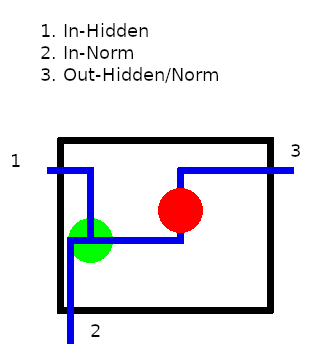
\includegraphics[scale=1.0]{diagram-rnn}
	
	\caption[Recurrent Neural Network]{RNN - 1 and 2 are inputs, 3 is the output.}
	
	%\addcontentsline{lof}{section}{Recurrent Neural Network}
\end{figure}

In our diagram the two inputs are labeled on the left side, and the single output does double duty as both the hidden state output and the value that the RNN surmises.

There are several designs for an RNN component. The inner workings of these components are what makes them different. In the example in the diagram the inner workings are very simple. Two paths, labeled as inputs, take data into the RNN. Their data is combined in the green circle. This combination is done with concatination and simple feed forward neural network components. The output from the concatination is passed through the red circle. This is a tanh activation operation that limits the output to values from -1 through 1. This tanh activation keeps the output within reasonable values. Finally the output is delivered outside the component to the program employing the RNN. In this diagram there is only one output. The single output would serve as both the hidden state output for that position in the chain, and also the data output component for that position in the chain.



\subsection*{Specific (GRU)}
A second type of RNN is the \ac{GRU}. GRU stands for `Gated Recurrent Unit'. A GRU has two inputs and two outputs. The formulas for a GRU, as outlined by Denny Britz in the website WILDML (Britz 2015)\cite{2015Britz}, are as follows.


$$ z =\sigma(x_tU^z + s_{t-1} W^z) $$  
$$ r =\sigma(x_t U^r +s_{t-1} W^r) $$  
$$ h = tanh(x_t U^h + (s_{t-1} \circ r) W^h) $$  
$$ s_t = (1 - z) \circ h + z \circ s_{t-1} $$  


The GRU has two inputs and two outputs. It also has two internal gates. One internal gate is the `reset' gate. This one determines how much of the previous input is combined with the new value calculated by the mechanism of the GRU. It is denoted as `$r$' above. Another internal gate is the `update' gate. The update gate decides how much new information is to be included in gate computation. It is denoted as `$z$'.

Here `$ s_t $' is the symbol for the output. `$h$' is the symbol for the `hidden output'. The two inputs are `$ x_t $' and `$ s_{t-1} $' . `$ x_t $' is the hidden state input. `$ s_{t-1} $' is the regular input for the RNN or GRU. Sigmoid activation is used on the two gates, while tanh activation is used to compute the hidden output.

In the last line, the regular output is determined using the `dot' product which is denoted with a circle, along with an addition operation. In the two gate formulas (the first and second) the output is determined as the sum of two matrix multiplication operations passed through sigmoid activation. This produces values in the range of 0 to 1.

Under most programming circumstances the GRU is not implemented by the average programmer. The programmer employs a language like python and a programming library like Pytorch or Tensorflow. The library then implements the GRU and makes it easy for the programmer to use that implementation.

\section{Sequence to Sequence}

Translating text from one language to another has become a common task for computers. The Sequence to Sequence architecture is often used today  for this purpose.

A naive approach to translation involves using a dictionary. You would encode each key as a word from one language and the value for that key would be the translated word in the target language. Of course this doesn't work, because different languages not only have different words for the same thing, but they also have different sentence structures for what might be similar concepts.

A better approach is sequence to sequence translation. A description follows with a section at the end for how training works.

In this approach we use recurrent neural networks to obtain our translation. Two recurrent neural network components are employed. One is responsible for the input language and the other for the output. Recurrent elements can remember sequences. 

Also employed are two vocabulary sets. One vocabulary is for the source language and another is for the target language. A table of word vectors the size of the input vocabulary is created and a maximum sentence length is picked. There is also a `hidden size', which is an important dimension in the model. In practice the hidden size could be 300 units and more for this kind of application.

First text is prepared for training. A text corpus with source and target pairs is chosen. Sentences in the source corpus are paired with sentences with the same meaning in the target corpus. Sentence length is observed and for all sentences shorter than that length a special `end-of-sequence' token is appended to all sequences in both languages.

Word vectors are created composed of floating point numbers. Each word in the vocabulary is translated to an integer which remains the same throughout the use of the translator. The word vectors are arranged in a table of floating point numbers with one dimension being the size of the input vocabulary and one dimension being the hidden size for the vector.

\subsection*{Recurrent Elements}
The recurrent unit in this case is a GRU. This stands for Gated Recurrent Unit. The GRU takes as input a single vector. It processes the vector and returns another vector. This could be
exactly the same as the input but is usually somehow changed. The input vector and the output vector have the
dimension of the `hidden size' mentioned above. Throughout the discussion of this model the hidden size will remain the same. The GRU also operates on two hidden states. One hidden state, a vector, is taken in and another hidden state, also a vector, is produced for output.

So far the model takes a word, translates it to an integer, and finds the vector in the word embedding table that represents that word. It does this for the first word and all subsequent words one by one. Then it gives the entire vector for a word to the GRU. The GRU takes the word and passes it to some inner components. It decides weather to return as output just the input or the input modified. This is what the GRU does internally.

We will use the metaphor of a chain when we describe input and output segments that are composed of GRU's. 

The input segments, composed of GRUs, take two input vectors and return two output vectors. One input is the vector from the embedding table. Another input vector is the hidden state. The hidden state is the same size as the input from the embedding table, but typically it comes from the previous input GRU. One output vector is like the word vector that's input to the GRU. One output vector is a hidden value.



The very first GRU in the input chain ignores the fact that the first word has no hidden value. It consumes the first word vector. Then it passes it's output to the next GRU in the chain. This GRU uses the output of the previous GRU as the hidden value. It also uses the vector for the second word. It passes it's important information to the GRU to it's right. Then the last GRU in the chain passes it's hidden state to the output chain.



A complicating detail is that although many GRUs are called for in the input chain they all use the same set of weights and 
biases. For this reason only a single input GRU is used for all of the words in practice. Outputs are calculated and then cycled around and fed with the next word from the sentence in vector form to the input of the GRU. 


The output chain is in charge of generating tokens that represent, in this case, the translation of the input in the output language. The output uses GRU segments also. The first hidden input for the first output cell is taken from the 
last hidden output of the last recursive unit of the input chain. It is important because it is the spot where a great amount of data is passed from the input chain to the output chain. 
The connection at this point is said to carry the `thought vector'. Most of the information responsible for translating one language to another is passed at this point.

The hidden values from the input section are passed to the first output GRU. It outputs the values that are later converted to the first word of the output. The first output GRU also has a hidden state. It passes the first word and the hidden state on to the second GRU.

The second GRU generates the second word and also its own hidden state. The second word is recorded and the word and the hidden state are passed on the the next GRU. This is repeated until a special `end-of-sequence' token is found or until the number of tokens equals the maximum number allowed.

\begin{figure}[H]
	
	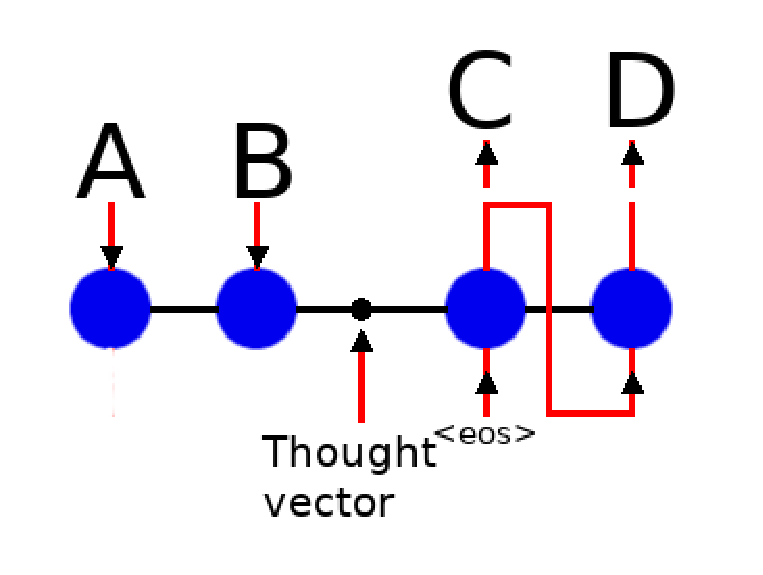
\includegraphics[scale=1.0]{diagram-nmt}
	
	\caption[Sequence to Sequence]{Seq2seq: A and B represent an input sequence and C and D represent the corresponding output.}
	
%\addcontentsline{lof}{section}{Sequnce to Sequnce}
\end{figure}

\subsection*{Output Tokens}
Each output we have is currently in the form of a vector. These vectors are a long string of floating point numbers, each one the dimensions of the `hidden size' mentioned above. What's done with them is they are converted to the dimensions of the output vocabulary. Then they are processed in what is called an `arg-max' function. This processing determines the index of the maximum value in the new vocabulary sized vector. This index allows the program to look up the corresponding word in the output vocabulary. This word is then used as the model output at that point in the output chain.

How does the model know what target vocabulary indexes go at what point in the output? For this we refer back to the corpus that we already have. One part of the corpus is the source language. The other part is the target language. A sentence is applied to the input and for that sentence an output is generated. The output is called a prediction. If the target and the prediction are not the same, the model must modify itself so that in the future they are.

There are some inherent problems. Because the output of a GRU is constantly being reused as the input, lots of data that might be useful to have is lost when the GRU churns through internal operations where several matrix multiplication operations are performed together on input. With every iteration more data is lost and so, for example, the effective length of the input and output sentences must be short. 

Another problem is that all input to be translated to target output has to be boiled down and 
passed to the output section through a small corridor the size of a typical word vector. This channel is sometimes referred to as the `thought vector.' Somehow all necessary information must be there. This also limits the length of the input and output vectors. It does help, when setting
up a model for later training, to make the hidden size larger, but it only helps so much. There is a point at which the benefit of increasing the hidden size is lost.

That ends our discussion of Sequence to Sequence Translation. This is how some computer models do language translation. Using arg-max is an example of a greedy approach. Another approach might use something like `Beam Selection' but we're not going to get into that here.


\section{Loss and Accuracy}

At first the prediction from a model is not very close to the desired output. The output is compared to the prediction and a `loss' is generated. `Loss' measures the difference between the predicted output and the target. A larger loss represents two values, prediction and target, that are further apart. The loss function must be chosen. 

%A typical loss function is 'Mean Squared Error' or MSE.

Another metric is Accuracy. `Accuracy' is a numerical representation of the difference between the desired output and the generated prediction. It is a percentage of the time that the output is exactly correct.

Getting a prediction, running input data through a neural network, is forward propagation.
Training, then, is a mathematical process involving backpropagagtion. Backpropagation identifies areas of the model weights that need to be modified in order to get the proper prediction in the future.

%\iffalse
In practice we take the derivative of the loss function in order to backpropagate. The derivative is manipulated with the learning rate and the original weight value is changed. The result is a set of adjusted weight matrices. When these matrices are used later they allow for better predictions. 
%\fi

This is done over and over with every source/target sentence pair. Slowly the model is changed and predictions start to match the target. That's training. The loss should decrease over time and the accuracy should increase.

There are several numerical metrics that we can record during training that tell us how our model is training. The loss, a mathematical calculation of the difference between the model's output and the predicted value, is mentioned above. Loss is an important number. Also accuracy is important. Accuracy is a mathematical calculation of the difference between the model's output and the value that output should be, but it focuses on the number of times the model comes out with a correct prediction verses how many output values there are in total.

\section{Attention Mechanism}

Here we consider a simple attention mechanism that is used in the Sequence to Sequence model by Inkawhich (2018)\cite{2018Inkawhich}. The concept for this attention comes from Luong et al (2015)\cite{DBLP:journals/corr/LuongPM15}.

Luong et al (2015)\cite{DBLP:journals/corr/LuongPM15} are interested in three kinds of calculation for their attention mechanism. The three methods use slowly increasing levels of complication. First they propose a method that just uses the dot product. Then they propose a method that just uses a field of weights. Finally they use a method that uses concatination, along with a field of weights and a pass through a tanh activation layer.

$$
\boldmath
score(h_t^ \text{,} \bar{h}_s) =
\begin{cases}
    h_t^\intercal \bar{h}_s & \text{dot} \\
	h_t^\intercal W_a \bar{h}_s & \text{general} \\
	v_a^\intercal \text{tanh}(W_a [h_t ; \bar{h}_s] ) & \text{concat}
\end{cases}
\unboldmath
$$

Here $h_t$ is the symbol for the output of the current decoder and $\bar{h}_s $ is the symbol for another output taken from the input encoder. This one is the entire set of encoder states. Inkawhich (2018)\cite{2018Inkawhich} uses the `dot' variety.

The formula is used after the decoder GRU calculates it's hidden state. It is below.

$$ 
\boldmath
score = h_t^\intercal \bar{h}_s 
\unboldmath
$$ 

Basically the output of the current decoder is transposed. Then it is multiplied by the hidden value from the entire set of encoder states. The result is multiplied by the GRU decoder output, and then passed through a tanh activation layer.

\section{Sequence to Sequence Chatbot}

Vinyals et al (2015)\cite{DBLP:journals/corr/VinyalsL15} make an interesting proposition. They say that it's possible to make what they call a Neural Conversational Model by constructing a Sequence to Sequence model, but instead of using two corpus from different languages a single language is used for both source and target.

Chatbots have for a long time been constructed using AIML. AIML, (Artificial Intelligence Markup Language) requires hand coding individual rules for every input and response. A Neural Conversational Model would not use those sorts of rules.

To create a model like this more is required than just a single input and output language. There must be a relationship between the source and the target. We want there to be a question-and-answer-like relation. Finding a corpus like this can be difficult.

It would be easy to duplicate the input source material in the target corpus. This would produce auto-encoding. The model would learn to repeat everything that was given to it in it's output. Though the model learns a task, it is not the dynamic task we want. Conversations, on the other hand, supply the relationship we are looking for. Starting with almost any question sentence in a conversation, the sentence following it answers the question posed. The latter fills a space that is opened up by the former. 

What would be a good candidate for this kind of verbal play? Vinyals et al (2015)\cite{DBLP:journals/corr/VinyalsL15} use a movie transcript dataset. Essentially they take movie dialogue and break it into sentences. Even numbered sentence are the source material, and odd numbered sentences are the target. Using this method there are times when the source and target are not from the same conversation, like times in a movie dialog when the scene switches from one locale to another. Comparing this, though, to the number of times that the two sentences are from the same dialogue, the movie transcript database serves very well.

Training for this model is relatively straight forward. There is a problem though. We can follow the loss and make sure it is decreasing, but the accuracy tells us nothing and in this case does not increase as we would like it to. The loss goes down but the accuracy does not go up.

\begin{figure}[H]
	
	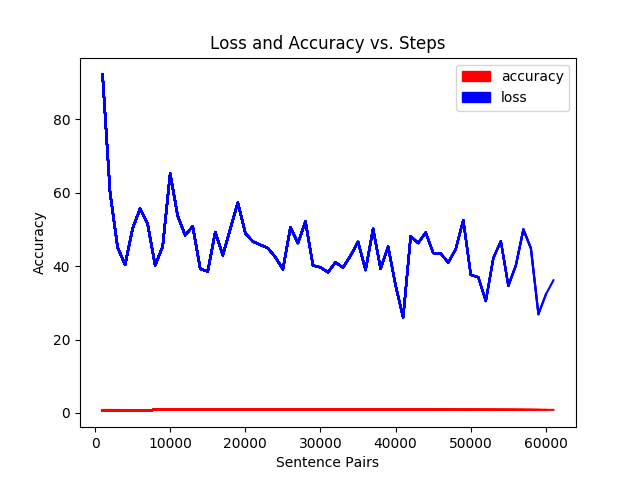
\includegraphics[scale=1.0]{Figure_1}
	
	\caption[Loss and Accuracy]{Loss and Accuracy: Red is accuracy and blue is loss.}
	
	%\addcontentsline{lof}{section}{Loss and Accuracy}
\end{figure}

This is because the source and target do not have the same meaning. The model does learn the task at hand but during training we have to ignore the accuracy. Success is usually measured by the accuracy of the holdout test set. Here we must measure the success with a subjective examination of the trained model.

We have to interactively give the model questions that we might ask someone that we are having a conversation with, and then see how it answers. Over and over we have to test the model. If we are satisfied with the answers then the training was a success.

\chapter{Transformers and The Generative Pre-training Transformer 2}

\chapter{Transformers and the Generative Pre-Training 2 Transformer}
\label{chapter-transformer}

\section{Transformer and Attention}

\label{transformer-intro}

The Transformer is a mechanism that is based entirely on attention. Strictly speaking, this is not the attention explored in the sequence-to-sequence model in Section \ref{section-gru-attention}, though there are some similarities. It is a model that uses no recurrent components.

Recurrent components have some negative qualities. They are hard to run with batch input data. In addition they do not work with very long data strings. 


Transformers use no Recurrent Neural Network components. Their operations can be parallelized so that large batches of data can be processed at once during the same time step. 

Longer sequences can be considered as well, so Transformer input can contain longer English language sentences and even paragraphs. 

Transformers are usually constructed on eight or more of these layers in the decoder and the encoder. One layer is discussed below.

\subsection{Byte Pair Encoding}

\ac{BPE} stands for ``Byte Pair Encoding.'' WordPiece is a particular implementation of BPE.

WordPiece is used by some Transformer systems to encode words much the way that Word2Vec does. Like Word2Vec, WordPiece  has a vocabulary list and a table of embeddings that maps one word, or token, to a vector of a given size.

WordPiece, though, handles Out Of Vocabulary (\ac{OOV}) words gracefully. It breaks large words into smaller pieces that are in the vocabulary, and has a special notation so that these parts can easily be recombined in order to create the input word again. Byte Pair Encoding doesn't use pre-trained word embeddings as do Word2Vec and GloVe.

For the Generative Pre-Training 2 transformer, a version of BPE is used instead of a vocabulary system like Word2Vec or GloVe. Some form of BPE is included in almost every Transformer type Neural Network model, so no decision needs to be made about what type of word embeddings to use.

\subsection{Attention}
Attention mechanisms are used in a similar way in three places in the Transformer model. The first implementation of Self Attention is discussed below. Each of these attention mechanisms is contained in a layer. There are typically the same number of layers in the encoder as in the decoder.

Input to the Transformer is composed of strings of words from a desired input language. Output is composed of words in a given language. Input words are treated very much the way that they are in sequence-to-sequence models. A word is translated to a number and that number indexes an entry in a word-to-vector table. From that time forward, a word is represented by a vector of floating point numbers. In a Transformer this word vector can be large. In the original paper, Vaswani et al \cite{Vaswani2017AttentionIA} use a vector size of 512. The discussion of Generative Pre-Training 2 will see vector sizes of 768 and 1280.

\begin{figure}[H]
	\begin{center}
		
		
		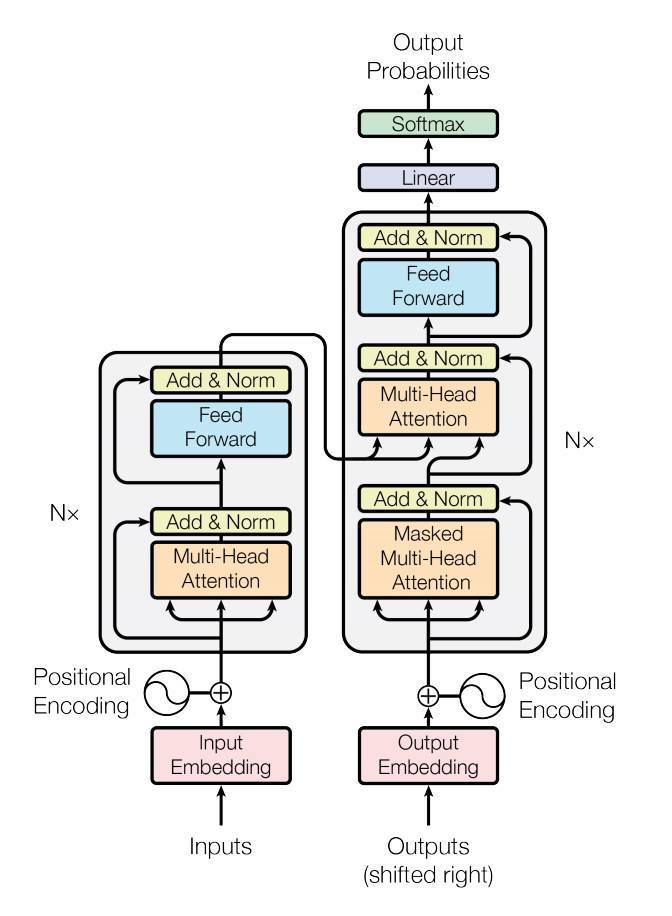
\includegraphics[scale=1.5]{diagram-mat04}
	\end{center}
	\caption[Transformer Encoder and Decoder]{Transformer Encoder and Decoder. - $Nx$ shows number of layers. (Data travels from the bottom to the top.) - Vaswani et al \cite{Vaswani2017AttentionIA}}
	
	
\end{figure}

\subsection{Encoder - Scaled Dot-Product Attention}

Each layer of the Transformer's encoder has a signature self-attention mechanism. This is possibly one third of the entire Transformer mechanism, but a variety shows up in the other two-thirds. 

Initially the input word vectors are converted to three other values. These vectors are similar to the input vector but they have a smaller dimensionality. Converting the word vectors in this way is accomplished by three simple matrix multiplication operations.

Figure \ref{diagram-mat-mult-01} shows a simple conversion of this type. In the diagram a conversion of a vector with dimension of 1x3 to a dimension of 1x2 is shown. In a real world example matrices are converted from a vector of 1x512 to 1x64, a division of 8.



\begin{figure}[H]
	\begin{center}
		
	
	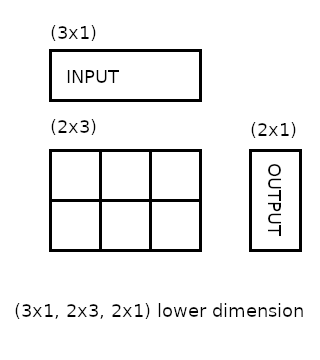
\includegraphics[scale=0.5]{diagram-mat01}
\end{center}
	\caption[Lowering Dimensionality]{Lowering Dimensionality}
	
	\label{diagram-mat-mult-01}
\end{figure}

In the Transformer, this conversion operation is probably the reason for the model's name. The input is \textit{transformed} to a lower dimension. 

The dimension of the starting vector must be preserved. The starting vector is of floating point numbers sized 512. After some processing the vector is converted to smaller 64 sized floating point numbers. The final output of the attention mechanism must be sized 512. %Before that is done the vector is processed at the smaller size of 64 floating point numbers. 

In this self-attention scheme three vectors are actually required. All three vectors are sized 64, and all three are converted by separate matrix multiplication operations. The weights to convert each of the three vectors are different. For this reason the new smaller vectors are all different.

The smaller vectors individually are called q, k, and v. They can also be referred to as larger matrices. The new vector matrices are denoted as Q, K, and V. Q stands for ``Query.'' K stands for ``Key.'' V stands for ``Value.'' The lower-case names refer to single vectors and the upper-case refer to matrices. These are essentially batches of input.

The Query value is multiplied by the Key values from all vectors in the input. This multiplication is ``dot-product'' multiplication. When it is done, all keys will have low output values, except those that are closest to the Query. Then the results are passed through a softmax function. When this is complete, there will be a single vector that is close to 1 and another group of vectors that are all close to 0.

The vector produced by multiplying the softmax with the V values of every word produces a single word vector that is close to its original value, and many others that are near zero.

This formula from Vaswani et al \cite{Vaswani2017AttentionIA} shows the process.

$$
\mathlarger{ \mathlarger{
Attention(Q,K,V)=softmax(\dfrac{QK^T}{\sqrt{d_k}})V
} }
$$

The value of $\sqrt{d_k}$ is used to limit the size of the $QK^T$ output. The $d_k$ is the dimension 512. Without this, the softmax function has to deal with much larger numbers. Smaller numbers for the softmax are preferred. $K^T$ is notation for the $K$ vector transposed.

The function can actually perform this on large matrices with high dimensionality, in parallel. This parallel matrix operation increases the speed of training.

In the triangle in the Figure \ref{attantion-7} the multiplication and selection that was just described is performed.

\begin{figure}[H]
	\begin{center}
		
		
		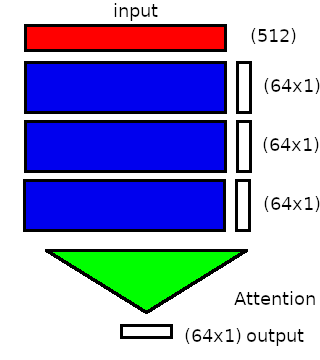
\includegraphics[scale=0.5]{diagram-mat04-64}
	\end{center}
	\caption[Attention Output]{Attention Output. (Data travels from the top to the bottom.)}
	
	\label{attantion-7}
\end{figure}




Finally the output calculated above must be returned somehow to the input dimensionality. This is accomplished by duplicating the procedure described eight times with eight separate weights. When this is done the output of the eight separate attention mechanisms is concatenated together, returning the output to the proper size.

This multi-headed approach allows different heads to learn different types of relationships and, then when they are grouped together, the learned relations are recovered and contribute to the output.

\begin{figure}[H]
	\begin{center}
		
	
	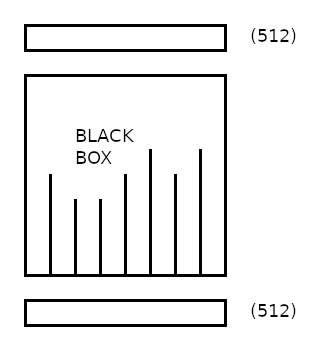
\includegraphics[scale=0.5]{diagram-mat02}
\end{center}
	\caption[Matching Input and Output]{Matching Input and Output. (Data travels from the top to the bottom.)}
	\label{attention-matching}

\end{figure}


Later the output is passed through a feed forward network. It is also combined with the original input again through addition. Then the output is normalized. This ensures that the values are all within reasonable ranges. This recombination of the attention output with the original output is done throughout each Transformer layer.

This describes the encoder section. There are two other attention segments. Together these two sections combine to form the decoder section. This is repeated for each layer.

\begin{figure}[H]
	\begin{center}
		
		
		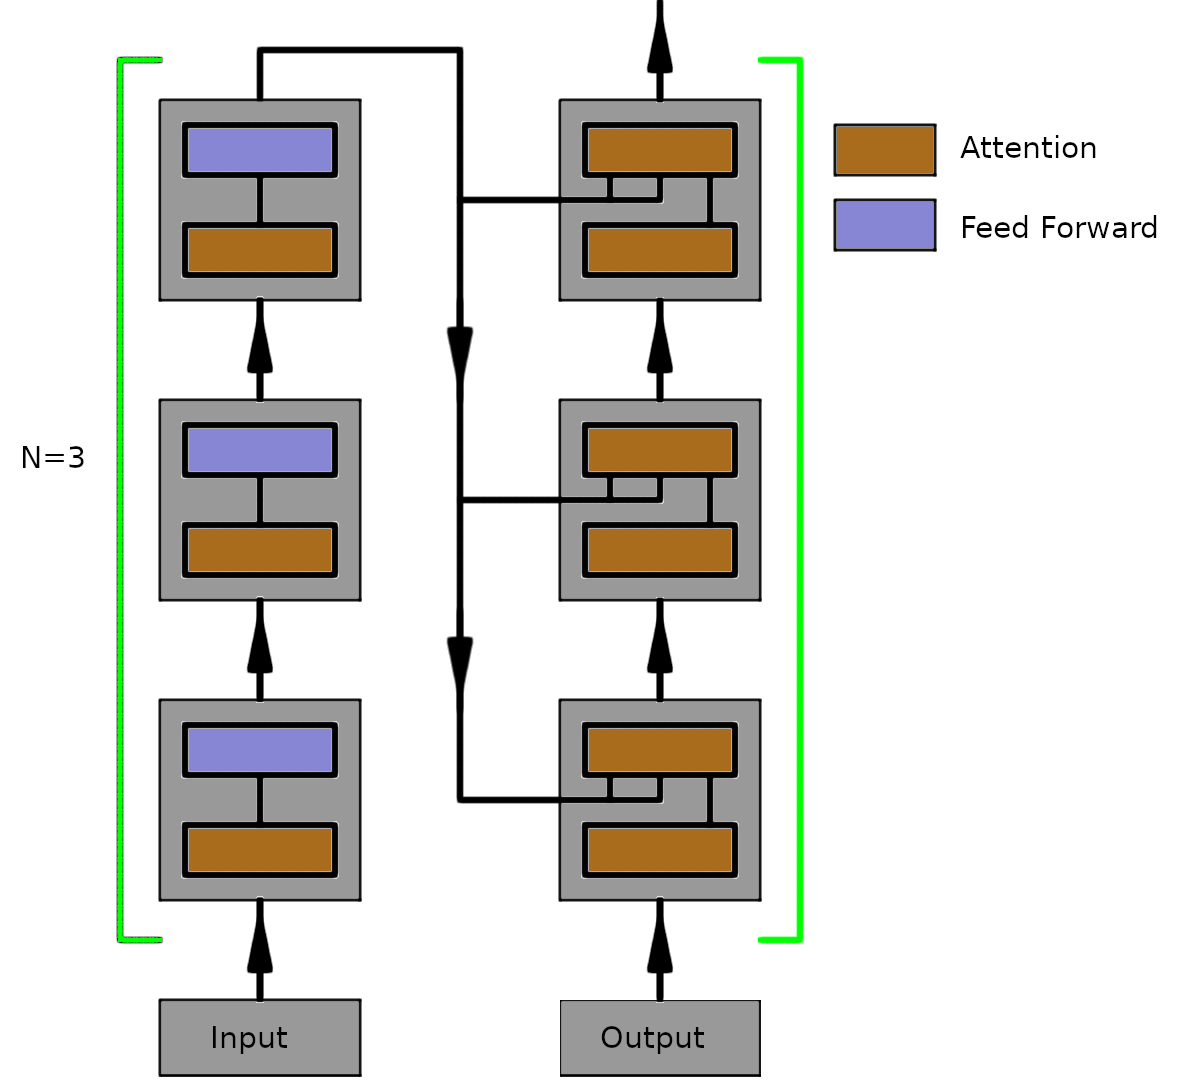
\includegraphics[scale=1.0]{diagram-flow1}
	\end{center}
	\caption[Transformer Encoder and Decoder Flow]{Transformer Encoder and Decoder Flow. - Three layers and data flow. (Data travels from the bottom to the top.)}
	\label{diagram-flow1}
	
\end{figure}

In the flow diagram, Figure \ref{diagram-flow1}, most sub-segments of the entire transformer are not described. The focus is the flow of data through the three encoder segments and the different flow of data through the decoder segments. The encoder is largely serial, while the decoder is serial and parallel. In fact each decoder segment includes a feed forward part, and all decoder and encoder parts include a residual connection where the input is added back to the output of the attention and feed forward segments.

The output of the encoder is a group of vectors the same size as the input sequence. They become the ``Key'' and ``Value'' batches below. The encoder section iterates once for every input data sequence.


\begin{figure}[H]
	\begin{center}
		
		
		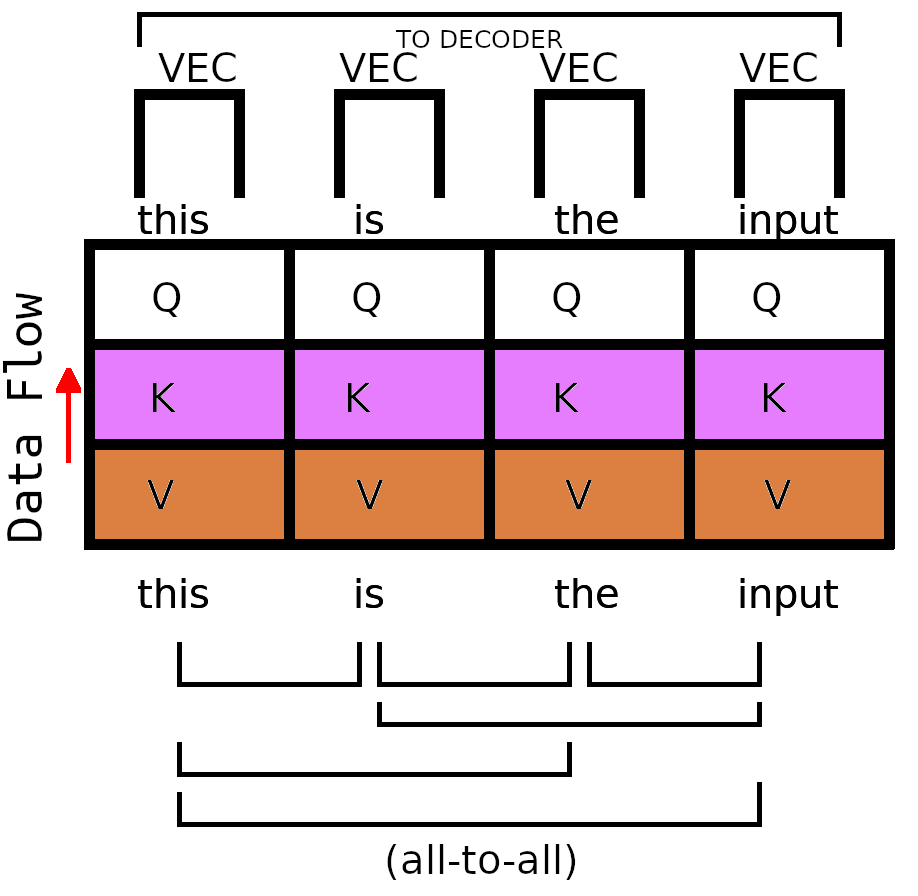
\includegraphics[scale=0.75]{diagram-graph-encoder-flow-b}
	\end{center}
	\caption[Encoder Attention Detail]{Encoder Attention Detail. (Data travels from the bottom to the top.)}
	
	
\end{figure}

\subsection{Decoder Attention I - ``Key'' and ``Value''}
The decoder is composed of two attention mechanisms and a feed forward segment at each layer. The result of the encoder's work is passed to the decoder and remains applied to one of the decoder's attention mechanisms in each decoder layer. In one attention mechanism of the decoder, the ``Key'' and ``Value'' matrices are imported from the encoder. 

While the encoder takes in the entire input and attends to whatever portion of that input it finds to be important, the decoder is interested in producing one output token at a time. The decoder section iterates once for every output word. Throughout this process the information from the encoder does not change.

In the flow diagram one layer of the decoder is illustrated.

\begin{figure}[H]
	\begin{center}
		
		
		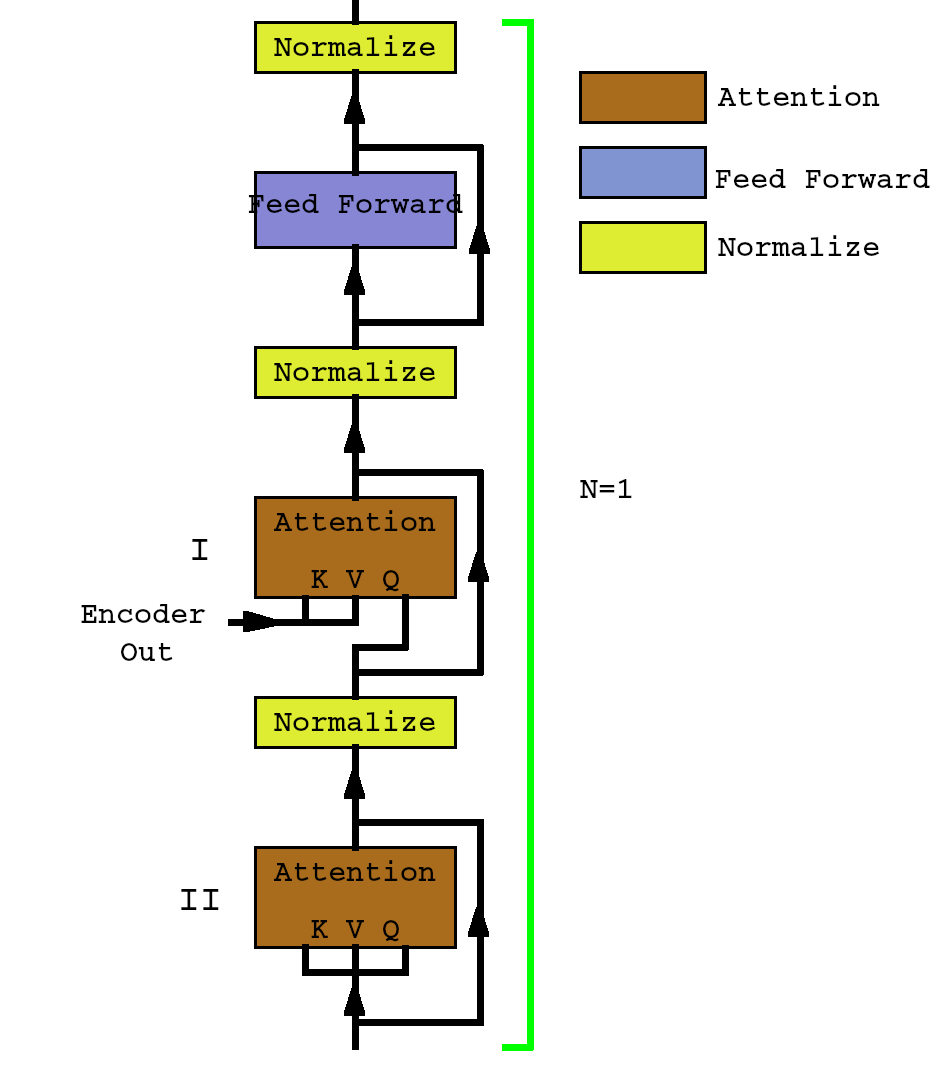
\includegraphics[scale=1.25]{diagram-flow-decoder02}
	\end{center}
	\caption[Decoder Flow]{Decoder Flow Details - ``I'' for encoder-decoder attention. ``II'' for masked decoder self-attention. (Data travels from the bottom to the top.)}
	
	
\end{figure}


Illustrated in the sequence-to-sequence discussion was the importance of the single ``thought vector.'' The Transformer can be seen as having a thought vector also. There is a corridor of data from encoder to decoder. It is composed of a sequence of vectors the size of the input sequence or sentence. It is larger, strictly speaking, than a single vector.

Two important smaller vector-sized inputs from the encoder are ultimately required in all layers of the decoder. They represent the ``Key'' and ``Value'' matrices from the thought vector. The matrices required are the size of the smaller reduced vector. The full sized vectors are transported from the encoder and are reduced dimensionally in the decoder layers to a sequence of two smaller matrices. 

These full sized vectors come from the last encoder layer's output. Typically there will be as many decoder layers as there are encoder layers. The output from the last encoder layer is applied to the ``Key'' and ``Value'' inputs of one of the attention mechanisms in all the decoder layers.
\begin{figure}[H]
	\begin{center}
		
		
		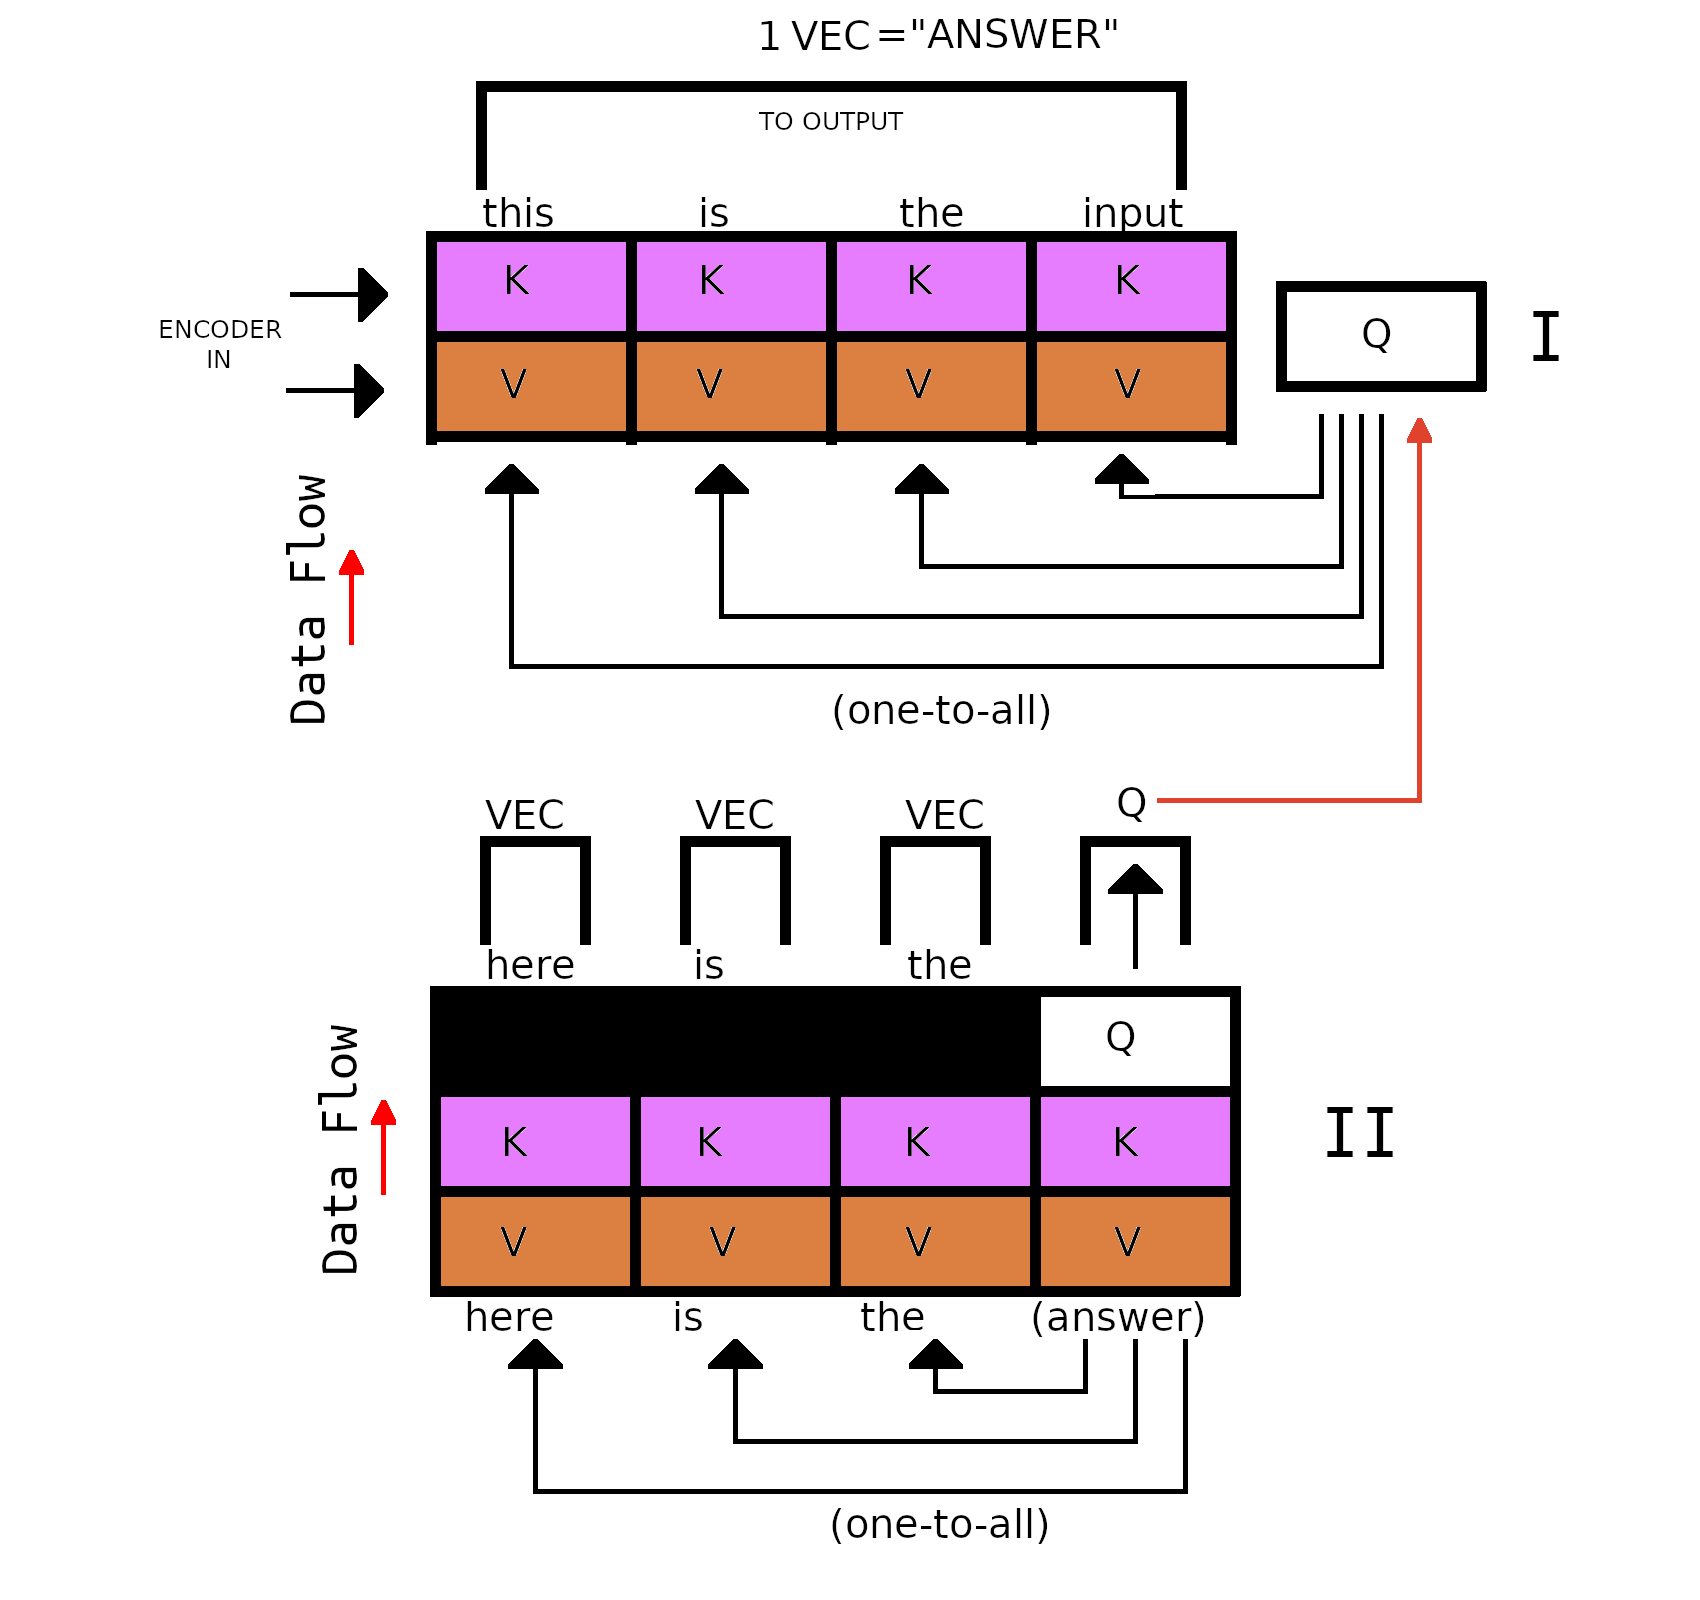
\includegraphics[scale=0.75]{diagram-graph-decoder-flow-c}
	\end{center}
	\caption[Decoder Attention Detail]{Decoder Attention Detail. (Data travels from the bottom to the top.)}
	
	
\end{figure}


\subsection{Decoder Attention II - ``Query''}
There is another attention mechanism in each decoder layer. It works solely on data from the decoder itself. It works very much like the attention mechanism from the encoder, but it attends to every word of output as opposed to the entire input sequence. It passes its output to the attention mechanism described above. This data is lowered in dimensionality and becomes the ``Query'' matrix for that mechanism. 

The ``Key'' and ``Value'' sequences from the encoder are a group of vectors the size of the input sequence. The ``Query'' matrix is the size of a single vector. This is because the decoder is interested in predicting one word at a time. This section produces a single vector as well.


\subsection{Decoder Attention II - Masking}
Input for the second decoder attention section is a group of vectors from the output generated thus far. During inference this output grows by one token with every pass through the decoder. This is how text is generated.

During training the second decoder section is masked. The mask prohibits the decoder from seeing parts of the target. This mimics the inference setup. In inference the decoder can only see up to the most recent word it has produced.

During inference the decoder produces a sentence one token at a time. Then it adds to that sentence, one token at a time, until the decoding is finished and something like English is produced. It can attend to any part of the output it has already produced. It is concerned with producing a single token at a time.

These tokens strung together are the output of the Transformer. This output should be readable. % English if the model output is set up for the English language.

More information about how this part of the decoder works can be found in Section  \ref{pre-trining-2-model}. Attention in this part of the Transformer is very similar to the GPT2.

\begin{figure}[H]
	\begin{center}
		
		
		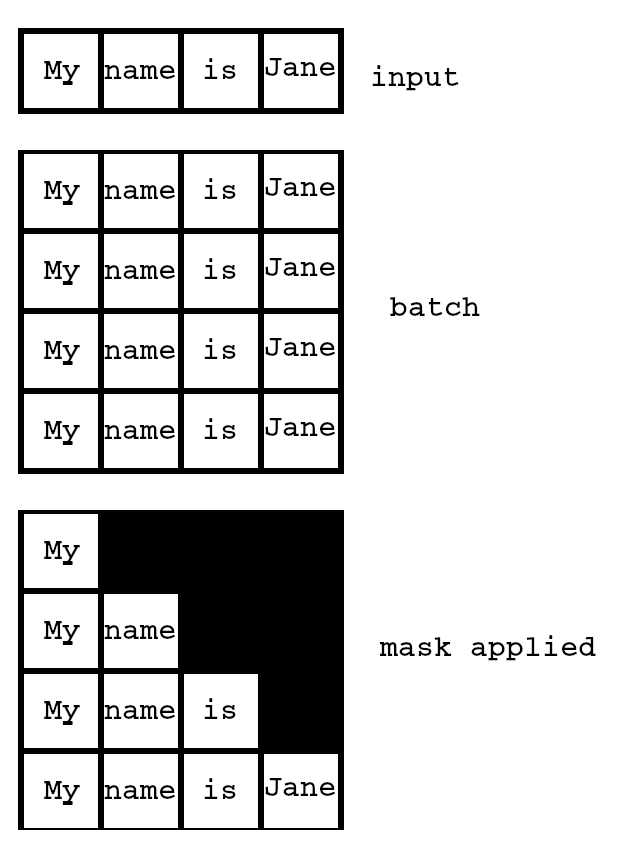
\includegraphics[scale=1.25]{diagram-mask01}
	\end{center}
	\caption[Decoder Mask]{Mask. - Decoder uses masked input during training.}
	
	\label{diagram-mask-01}
\end{figure}



%\subsection{Transformer - General}
\subsection{Input - Positional Encoding}
The input of the Transformer encoder and decoder layers employ not only a word vector table, but also a positional encoding scheme. The model adds sine and cosine patterns to the input vector that it can then use to learn the position of words in a sentence. 

Words that are early in the sentence have a certain appearance and words later on appear differently. The encoder and decoder use the sine and cosine waves to impart this information onto the sentence sequence. 

\subsection{Output - Feed Forward Network}
At the output of the last layer of the decoder, the output vectors are processed through a linear matrix which increases the vector's dimensionality, so that the output vector is the size as the output vocabulary dimensionality. After the linear matrix the vector is processed by a softmax function. Then the highest floating point value in the new larger vector is the index of the chosen output word.


\subsection{Visualization - Transformer}

A colorful chart is used to visualize what is happening during inference. This chart illustrates how each word attends to all the other words in the input text.

\begin{figure}[H]
	\begin{center}
		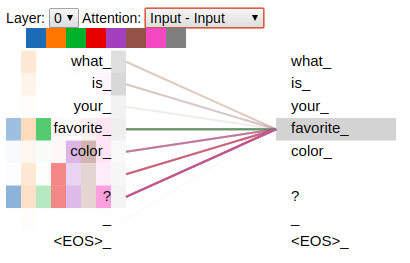
\includegraphics[scale=2]{Figure_3}
		
		
	\end{center}
	\caption[Visualized Attention Transformer]{Visualized Attention -- ``favorite'' shows attention to some but not all words in the sentence.}
	
	
\end{figure}

It is significant that words like ``what'' and ``your'' do not have strong attention to other words in the text. In a chart like this one they would show no colors on the left and light colored lines connecting the right to the left.

This diagram is from the Transformer with the larger hyper-parameter set that is described in Chapter \ref{chapter-approach-to-study}, trained on the movie dialog corpus.


\section{The Generative Pre-Training 2 Model}

\label{pre-trining-2-model}

``Generative Pre-Training 2'' is a large model. It is based on the Transformer from Vaswani et al \cite{Vaswani2017AttentionIA} but there are some major changes. The model uses the decoder portion of the Transformer without the encoder. There are other changes to the output layers. Furthermore it is pre-trained and downloadable.

We use the GPT2 model to create some of our chatbots.


\subsection{Pre-Training}
In Pre-Training the authors of a model train an instance and then make the model available to the user on-line. This is helpful for the average programmer interested in Neural Networks. Training an instance of the Transformer model can use computational resources for days, and require hardware that is costly. Usually the cost of producing a trained model is prohibitively expensive.

After acquiring a trained model, programmers go on to adjust the model to their task. Adjusting a pre-trained model to a given task is called ``Transfer Learning.'' Many tasks lend themselves to Transfer Learning. Conceptually a model can be fine-tuned to many problems. % and many problems can be addressed with good results after only modest fine-tuning.


\subsection{General}
\ac{GPT2} still uses Scaled Dot-Product Attention. A model diagram is taken from Radford et al \cite{radford2018improving}. 

\begin{figure}[H]
	\begin{center}
		
		
		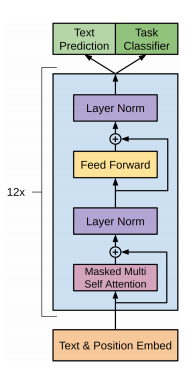
\includegraphics[scale=3.0]{diagram-mat05}
	\end{center}
	\caption[Generative Pre-Training 2 ]{GPT2 - Radford et al \cite{radford2018improving}. (Data travels from the bottom to the top.)}
	

\end{figure}

There are several sizes of pre-trained GPT2 models, all rather large. The smallest model has 12 layers, while the Transformer model in the example from Vaswani et al \cite{Vaswani2017AttentionIA} uses 8 layers. This model also has a hidden dimension of 768, not 512. With 8 heads this leaves a smaller dimensionality of 96 at each attention head. 

%The GPT2 models input and output text sequences.


\subsection{Training}

The GPT2 model is trained on text from the web, specifically Reddit. The goal for training is to show the model part of a large piece of text and then to have the model predict the next word. A mask is used in the Self Attention segment of the model during training.

%For this task the mask is important. Training could consist of incrementally showing a model text at different states of completion and then asking it to predict the next token. In this kind of arrangement the batch sizes would be shorter and focus on each word. 

Training could present the model with the text in complete form and have the model look at it through a mask. A mask is visualized in Diagram \ref{diagram-mask-01}.

Each word would have an opportunity to be focused on as the ``next'' word. A boundary is formed between the last word and the masked area to its right. The boundary between each word and the one that follows it is examined. The model can still be trained on large batches in parallel. Words to the right of the last word and the particular boundary being examined are not available to the model.

Training is done by the developers of the model and the authors of the paper. The model is too big for individuals to train from scratch. 

\subsection{Inference}

In this example creating ``conditional samples'' are discussed, in contrast to creating ``unconditional samples.'' Conditional samples rely on an input sequence for generating output. Unconditional samples have no input specified. %A mask is not used during inference.

First a series of input tokens must be selected for the example. This series of tokens is generated from an English sentence. The sequence used will be ``Good day'' for this example. The words in the sequence translate into single tokens in the corpus. An input word may be made up of several tokens, but that should not be the case in this simple example.

The input context for GPT2 models is 1024 tokens. Here the input tokens, ``good'' and ``day,''  take up two spots in the input area. They are followed by an end-of-sequence token. Together they take up three spots. At that time there are 1021 spots left in the input area.

The first words are converted to tokens and are passed through the embedding matrix where they are converted to vectors. Positional encoding patterns are generated for each of the three vectors. These positional encoding patterns are created from sine and cosine waves that are concatenated together. They are added to the input tokens.

The model starts at the fourth location and attempts to generate the next token. The entire model is at this moment addressing the task of generating the next token.

One of the important processes that the input goes through is the Scaled Dot-Product Attention. This is performed at each layer. There are 12 layers in the 117M model.

All three tokens are converted to smaller vectors for each layer. Then the third vector, for the end-of-sequence token, is treated as the ``Query.'' The matrices for the ``Key'' and ``Value'' are assembled from the words in the input. This is done for all of the heads of each individual layer.

At this time, the model is making the transition from the third spot to the fourth spot.

The third word ``Query'' vector, the end-of-sequence, is compared to each other previous word ``Key'' vectors using dot-product multiplication. Then the result is Softmaxed, producing a single vector that is close to 1 and a group of all other vectors that are closer to 0. The result of that is multiplied by all of the three ``Value'' vectors. A single result is found in this way.

The output is concatenated together at each layer across all the heads at that layer. Ultimately the output is recombined with the input. There are also components in each layer that do normalization.

Ultimately an output vector is produced that represents what the next token should be. %This vector is converted into a size equivalent to the size of the vocabulary. Then the model can use a method to choose a word from the vocabulary. 

%Frequently, the model looks to the largest floating point number and its association with a word in the vocabulary.

The new token is placed in position four. The first three tokens are left as they are and GPT2 goes back to the start and now looks at the first four tokens as input. It will try to generate the fifth token.

The model will continue to try to generate tokens until the input area is filled and there are 1024 tokens, or a special ``end-of-sequence'' token is generated. The output could be anywhere from 1 to 1021 tokens. This is because the input area starts with a dimension of 1024, and there are three tokens in the original input sentence.


\begin{figure}[H]
	\begin{center}
		
		
		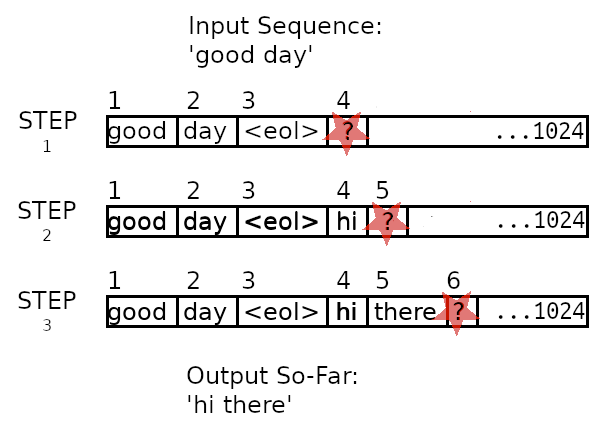
\includegraphics[scale=2.0]{diagram-inference-02}
	\end{center}
	\caption[Generative Pre-Training 2 Inference]{GPT2 - Inference Progress}
	
	
\end{figure}

\subsection{Corpus}
The GPT2 models are trained on a corpus called WebText, a 40GB corpus taken from the Reddit web site. All the material comes from before 2017 and all has a ``karma'' rating of three or better. ``Karma'' is a rating system used internally on Reddit. 

%As with the decoder layer of the Transformer model, the GPT2 model concerns itself with generating words that are later strung together to make sentences or paragraphs. During training the model uses a masking scheme so that input can be parallel-ized. During inference output cannot be parallel-ized, so during inference output must focus on one example at a time.

\subsection{Releases}
In their paper, Radford et al \cite{radford2019language} showed that their model could generate text from a seed sentence or paragraph. At that time the case was made that the largest ``Generative Pre-Training 2'' model should not be released because of its ability to generate text that might fool humans into believing that another person was responsible for the text. Later the larger model was released to the public.

\begin{center}

\begin{tabular}{lrll}
	Size & Parameters & Layers & $d_{model}$ \\
	\hline
	small & 117M       & 12     & 768          \\
	medium & 355M       & 24     & 1024         \\
	large & 774M       & 36     & 1280         \\
	x-large & 1.5B     & 48     & 1600 \\
	xx-large & 8.3B   &  72 &   3072 
\end{tabular}

	
\end{center}
\addcontentsline{lot}{section}{GPT2 Size Overview}

When the first ``Generative Pre-Training 2'' models were released there were three of them. Later two more were trained. The final xx-large model was trained by NVIDIA Applied Deep Learning Research \cite{2019NVIDIAadlr} and was not released to the public.

The ``Generative Pre-Training 2'' models also work in many circumstances in ``zero-shot'' mode, with no extra training to make the model suit the task. It is used ``as is.''

For the chatbot the model using 117 million parameters was successful. Some programming was required to make the model output look like chatbot output, but the model itself was not modified.

Tests were done on both the small and large models. When the larger 774M model was released it was used as a substitution for the 117M model. The test worked, and returned answers that were more well formed than the small model. The larger model does not fit on a Raspberry Pi and so it was not employed here on a permanent basis. %Using the extra large 1.5B parameter model in a chatbot was not attempted at first.

\subsection{Application Details}
The 774M model is described in Radford et al \cite{radford2019language} and the accompanying blog post. The model is trained on English without a stated problem, however large neural network models are usually trained for a stated problem. Rather famously this model is used after training to generate English language text. The model takes input from the user, a premise or summary of what is to be generated. The model also takes as input a number called the ``temperature.'' Then the model generates output. As the ``temperature'' is set higher, the output is more fanciful. There is also a tune-able parameter for the output length. 

%Given the ability of the model to invent content, it was determined by the authors that the `large' model should not be released to the public at first. Months later the `large' model was released. 

For the chatbot the temperature is set to a low number. The length of the output is set to a sentence-length number of tokens. Then as input the output from the speech-to-text translator is used.

The output is not immediately useful. Traditional programming and string manipulation are employed to clean the output and render a short single sentence. %This is the output.

Because the input is meant to be a number of sentences and, because the architecture is Transformer-based, more information can be added to the input string. In this respect the model acts to summarize the input. 

A set of three or four sentences is included with every input string. They suggest the time, the bot's name, and the bot location and occupation. The chatbot summarizes the input. If the information is relevant then it is used by the model as output. %Making this possible is the fact that a Transformer can accept much longer input strings than a Gated Recurrent Unit, and generate much longer output strings.

Surprisingly the chatbot answers most of the questions in the first person. It is felt that WebText, the Reddit corpus, has many examples of sentences in the first person.

\subsection{Visualization - GPT2}

During inference the Scaled Dot Product Attention in the GPT2 focuses on certain words as it processes input text. Here, the word ``favorite'' shows a relationship to many of the other words in the text.  

\begin{figure}[H]
	\begin{center}
		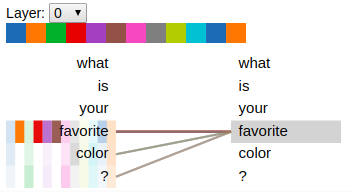
\includegraphics[scale=2]{Figure_4}
		
		
	\end{center}
	\caption[Visualized Attention GPT2]{Visualized Attention GPT2 -- ``favorite'' shows attention to some but not all words in the sentence.}
	\label{diagram-vis04}
	
\end{figure}

The phrase ``What is your favorite color?'' is often answered with ``I love the colors of the rainbow.'' This answer does not mention a specific color, as one might expect it should. Figure \ref{diagram-vis04} might support this observation because ``color'' on the left is not heavily highlighted. Words like ``what'' and ``your'' are barely considered at this head at all. 



\chapter{Experiments}

\section{Approach to the Study}

Several neural network models are used in the project. One is the sequence to sequence model and another the transformer model for a generative chatbot and finally the Generative Pre-training Transformer 2 model.

We will not try to rewrite the transformer or GPT2 model ourselves.

In this project we attempt to load as much of our chatbot code onto a Raspberry Pi as possible. We have trained models using the pytorch and tensorflow libraries. These models are responsible for taking in English sentences and producing English output. There is another part of the typical Raspberry Pi setup that includes another neural network component. Speech to text models, which our application requires, rely on large neural network resources. For this purpose we use speech to text resources supplied by Google on the google cloud. To include speech to text libraries locally on the Raspberry Pi would be too costly in computation time and resources like RAM. It would also be complicated to implement technically. It could easily comprise an entire project on its own.

Unfortunately the speech to text resources supplied by Google cost money. To use the service you need to have a billing account with Google.

The speech to text service used on the project and the memory limitations on the Raspberry Pi leads one to ask the question weather the neural network responsible for the chatbot function could not be servable from some faster machine located somewhere on the internet. At this time we are not interested in serving these resources. It would entail two calls from the Raspberry Pi for every sentence. This complicates things and also has a time overhead. 

Also, we have several models that we want to test. To test them all would require several servers. In addition we use both Pytorch and tensorflow. Tensorflow has `tensorflow-model-server' for serving models, but Pytorch has no equivalent.

It is important to note that the large Generative Pre-training Transformer 2 model specifically could be served from a remote computer and it would operate faster. Currently on the Raspberry Pi decoding a single sentence takes approximately 13 seconds. Even so, we prefer to install our trained models on the Raspberry Pi directly.

\section{Model Overview}

%\begin{center}

\begin{table}[h]
	
	\begin{center}
		
		
		\begin{tabular}{lllllll}
			
			Model Name    & File  & RAM  & RAM  & Pretrained  & Hand & Raspberry \\
			&  Size & Train   & Interactive   & Weights & Coded &   Pi \\
			\hline
			\hline
			Seq-2-Seq/Tutorial & 230 M     & 1.1 G & 324 M & NO                 & NO  &   3B \\
			Transformer/Persona   & 25 M      & 556 M & 360 M & NO         & PARTIAL  & NONE \\
			Transformer/Movie   & 550 M      & 6.5 G & 1.5 G & NO         & PARTIAL    & 4B  \\
			GPT2 small*   & 523 M     & 5 G   & 1.5 G & YES                & NO     &  4B \\
			\hline
		\end{tabular}
		
		* a large GPT2 model exists, but it is not small enough to fit on a raspberry pi.
		
		
	\end{center}
	
	\label{fig:modeloverview}
	\addcontentsline{lot}{section}{Model Overview}
\end{table}


Here we itemize a short description for each row in the table.

\begin{itemize}
	\item \textbf{Sequence to Sequence - Tutorial} This model uses the sequence to sequence architecture and the Gated Recurrent Unit component. We hand-coded our own example of this model but it performed poorly. This model is the slightly modified version of the Sequence to Sequence model based on the tutorial from Inkawhich et al\cite{2018Inkawhich}. It actually uses the Movie Dialog corpus. 
	\item \textbf{Transformer - Persona} This model uses a Tensorflow Transformer architecture. There was some coding involved to get the model to interface with the text-to-speech and speech-to-text libraries. There was also some coding to load our own corpus data during training. The model parameters describe a rather small model. This model also uses the Persona Dialog corpus. It is not on a Raspberry Pi board.
	\item \textbf{Transformer - Movie} This model is based on the transformer model above but uses the Movie Dialog corpus and a parameter set that is larger. In many ways this model is bigger than the model that uses the Transformer and the Persona corpus.
	\item \textbf{GPT2 small} This model was downloaded from the internet. It fits on a Raspberry Pi 4B with the 4GB RAM option. Some modification was made so that model output was suitable for our purposes.
\end{itemize}



\section{Setup}

We use linux computers, sometimes with \ac{GPU} hardware for parallel processing. We also use the Python programming language. Code from this project can be run with the 3.x version of Python.

When the project was started we did some programming with Keras using Tensorflow as a backend. Keras was later discarded in favor of Pytorch and Tensorflow. Pytorch as a library is still under development at the time of this writing.

Some of the Generative Pre-training Transformer 2 code uses Pytorch. Some of the Transformer and Generative Pre-training Transformer 2 code uses Tensorflow. There is a repository on Github that has the GPT2 trained model using Pytorch instead of Tensorflow.

We use github as a code repository. Code corresponding with this paper can be found at: \href{https://github.com/radiodee1/awesome-chatbot}{https://github.com/radiodee1/awesome-chatbot}
. 

As a coding experiment we rewrite the code for the sequence-to-sequence Gated Recurrent Unit model. We have varying amounts of success with these experiments. We do not rewrite the Generative Pre-training Transformer 2 code from the Tensorflow or Pytorch repository.

\section{Graphical Processing Unit vs. Central Processing Unit}

A CPU has a number of cores, a number usually between 2 and 16. A CPU is designed, though, to execute one command at a time. This allows for a logical program that can be executed. A CPU has limitations when it comes to executing matrix multiplication. Matrix multiplication using a CPU can take a long time.

GPUs, Graphical Processing Units, have the ability to address tasks like matrix multiplication with many more processing units at once. The GPU speeds up parallel processing and have a benefit to neural networking training tasks that the CPU doesn't have.

Unfortunately state of the art neural network models are larger than the capacity of a single GPU. Some models are trained on many GPUs simultaneously. It is not uncommon for a model to train on a computer with eight GPU cards for many days. Training these models is prohibitively expensive for the average programmer. It is possible to rent time on Amazon Web Services or Google cloud with well outfitted computers but this can be costly.

This sort of situation is addressed partially by the Transfer Learning scheme. In Transfer Learning someone else trains the model and makes the trained version accessible to the public. Then the average programmer downloads the model and fine tunes it to their task.

This would be fine if there were a model for every task. Though many models exist there seems to be many tasks that are not addressed. It seems that there is often the opportunity to train a large model by utilizing the CPU and training for long periods of time. This arrangement is not advised for the sort of experimentation where it is not a certainty that the output will be successful. If the goal is to do something that might not work, don't undertake it or use a Amazon or Google computer. If success is assured and time is plentiful continue with the CPU.

In this paper the GRU based Sequence-to-sequence model and the Tensorflow based Transformer model were trained from scratch on a CPU laptop. In the case of the Transformer, several days were required for training. In the GRU example the model trained in less than an hour.

\section{Raspberry Pi}

A Raspberry Pi is a small single board computer with an `arm' processor. There are several versions on the market, the most recent of which sports built-in wifi and on-board graphics and sound. The memory for a Raspberry Pi 3B computer is 1Gig of RAM. Recently available, the Raspberry Pi 4B computer can sport 4Gig of RAM.

It has always been the intention that at some time some chatbot of those examined will be seen as superior and will be installed and operated on a Raspberry Pi computer. If more than one model is available then possibly several models could be installed on Pi computers.

For this to work several resources need to be made available. Pytorch needs to be compiled for the Pi. Speech Recognition (\ac{SR}) and Text To Speech (TTS) need to work on the Pi.

For one of the transformer models to work Tensorflow needs to work on the Pi.

All the files that are trained in the chosen model need to be small enough in terms of their file size to fit on the Pi. Also it must be determined that the memory footprint of the running model is small enough to run on the Pi.

In the github repository files and scripts for the Raspberry Pi are to be found in the \textquoteleft bot\textquoteright{} folder.

Early tests using Google\textquoteright s SR and TTS services show that the Pi can support that type of functionality. 

Google's SR service costs money to operate. Details for setting up Google's SR and TTS functions is beyond the scope of this document. Some info about setting this up can be
found in the README file of this project\textquoteright s github repository.

The pytorch model that is chosen as best will be trained on the desktop computer and then the saved weights and biases will be transferred to the Raspberry Pi platform. The Pi will not need to do any training, only inference. 

\section{Tensorflow vs. Pytorch}

Tensorflow is a Google library. Pytorch has it's roots with Facebook. Both run in a Python environment. The learning curve for Tensorflow is steeper than for Pytorch. Pytorch offers the programmer python objects that can be combined to create a neural network. Tensorflow has different pieces that can be combined, but they cannot be examined as easily at run time.

Tensorflow has a placeholder concept for inputting data and getting back results. You set up these placeholders at design time. They are the only way of accessing your data at run time.

Pytorch objects interact with Python more naturally. You can use print statements in your code to show data streaming from one object to another. This is possible at run time.

In favor of Tensorflow, it has a good tool for visualization which can print out all kinds of graphs of your data while your model trains. It is called Tensorboard.

\section{Speech and Speech To Text}

Google has python packages that translate text to speech and speech to text. In the case of text to speech the library is called `gTTS'. In the case of speech to text the library is called `google-cloud-speech'. 

The gTTS package is simple to use and can be run locally without connection to the internet. The google-cloud-speech package uses a google cloud server to take input from the microphone and return text. For this reason it requires an internet connection and an account with Google that enables Google cloud api use. Google charges the user a small amount for every word that they translate into text. 

Both of these resources, the text-to-speech and speech-to-text, work out of the box on the Raspberry Pi, but configuring speech-to-text for the Pi is not trivial. The user must register a billing account with Google cloud services. In return for this registration the user is able to download a json authentication file. The file must be copied to the Raspberry Pi. 

Furthermore an environment variable must be set that points to the authentication file. The variable is called `GOOGLE\_APPLICATION\_CREDENTIALS'. This environment variable has to be set up before the respective model runs. When the model is launched on startup it may not be launched as a regular user. The model may be launched as, for example, the root user. Somehow the environment variable must be set along with the launching of the neural network model.

The operating system on the Raspberry Pi is based on Debian Linux. In this operating system there is a file which is run immediately after the basic system starts up. This script is called `\textbf{/etc/rc.local}'. It is sufficient to put the environment variable there and follow it with the launching of the model. To ensure that the process goes without a hitch, we attempt to combine the setting of the environment variable with the launching of the program in a single line of code.

\section{Corpus Considerations}

We have collected several data sets for the training of a chatbot model. Firstly we have a corpus of movie subtitles. Secondly we have a `JSON' dump from Reddit that is downloadable.  This is not the same Reddit data that the authors of GPT2 use. Finally we have the corpus described by Mazar{\'{e}} et al\cite{DBLP:journals/corr/abs-1809-01984}. This final corpus is designed for training the chatbot task specifically. This is referred to as the Persona corpus.

The movie corpus is medium sized and the Reddit `JSON' download is large and filled with hyperlinks and sentence fragments. 

At the time of this writing we are using the movie subtitles corpus and the Persona corpus. We use the movie corpus because it is smaller. Both the movie corpus and the Reddit corpus are described as noise filled, so it is likely that neither one is perfect for the training. The movie corpus is easier to deal with if we are training on a single processor. In the future if we can train in a faster environment the Reddit corpus might be superior.

For the Persona corpus the text is organized into `JSON' objects. There are several different repeated labels. Some of the text is meant to be used in question and answer pairs. There is also some very specific information there that is not organized in this kind of pattern. When we take apart the Persona corpus we find that the sentences labeled with the `history' tag are most suited to our task. We record these values only and discard other labels.

\section{ARMv7 Build/Compile}

\subsection*{Pytorch `torch' Library 1.1.0 For ARMv7}
We compile the Pytorch library for Raspberry Pi. We use several virtualization techniques to do this compilation. The result of those efforts is a Pytorch python 3.7 library for the Raspberry Pi.

On their web site Milosevic et al\cite{2018Milosevic} compile Pytorch 1.1.0 for the Raspberry Pi. We follow their instructions closely. We are able to build the package for the ARMv7 platform.

The instructions called for constructing a change-root environment where a Fedora Core 30 linux system was set up. Then the ARMv7 system was used in the change-root environment to compile the Pytorch library for the 1.1.0 version.

The production laptop used for development ran Ubuntu linux. For this reason a Virtualbox emulation was set up with Fedora Core 30 on it. Inside that emulator the change-root environment was set up. The library was compiled there successfully. 

There are two problems with the resulting built python package. Firstly there is an error in python when importing the torch library. The error reads `ImportError: No module named \_C'. 

After some research it is clear that the build process for ARMv7 creates some shared object files that are misnamed. A fix is to find the misnamed files and make copies of them with a suitable name. The same outcome could be assured by making symbolic links to the misnamed files with proper names.

There are three files misnamed. They can be found at `\textbf{/usr/lib/python3.7/site-packages/torch/}'. They are named with the same convention. They all have the ending `.cpython-37m-arm7hf-linux-gnu.so'. We want to rename them with the much shorter `.so'. The files are then named `\textbf{\_C.so}', `\textbf{\_dl.so}', and `\textbf{\_thnn.so}'.

This takes care of the `ImportError'. The second problem is that the version of GLIBC in the change-root environment does not match the GLIBC library in the Raspberry Pi Raspbian distribution. This produces the following error: `\textbf{ImportError: /usr/lib/x86\_64-linux-gnu/libstdc++.so.6: version `GLIBCXX\_3.4.26' not found}'.

This is solved by rebuilding the package with Fedora Core 29 instead of 30. 
 
\subsection*{Pytorch `torch' Library 1.4.0 For ARMv7}
We recompile the Pytorch library for the Raspberry Pi. We use debian virtualization techniques for the compilation. Because ubuntu is a debian derivative it is not necessary to run the process in a Virtualbox container. 

In addition to this, the files created by the compilation are properly named. There is no need to go to the directory `\textbf{/usr/lib/python3.7/site-packages/torch/}' to change anything. 

The time spent compiling the software is approximately 5 hours. Time spent with the Virtualbox container was easily twice that. The time spent on the Raspberry Pi executing a single Generative Pre-training Transformer 2 question and answer remains about 13 seconds, so there was no gain in that respect.

There were several small hurdles to completing the compilation. Firstly the `debootstrap' command needed to be employed at the start. Debian Stretch was used as the host operating system. It was felt that if it was used that the GLIBC compatibility problem would not be faced. This turned out to be the case.

There are some dependencies that need to be installed on the `chroot' environment for Pytorch to compile. One of these is that is important is `libblas3.'

Then Python 3.7 needed to be built on Stretch. The Stretch program repositories use Python 2.7 and 3.5 . The Raspbian operating system on the Raspberry Pi 4B is based on Debian Buster and uses Python 3.7. After compiling Python 3.7 the Git program needed to be compiled from scratch. Git on Stretch has a issue that is fixed upstream, but we want to use Stretch because of the GLIBC issue. Instead of using the upstream fix, we compile Git ourselves.

It is conceivable that the GLIBC issue would not be important if the `chroot' environment used Debian Buster, since that is the basis for the current Raspbian operating system. The Stretch operating system solution works though.

Finally the Pytorch program needed to be built. We disable CUDA and distributed computing as neither exists on the Raspberry Pi.

\subsection*{Docker Container `tensorflow-model-server' For ARMv7}
The Google machine learning library for python uses a standalone program called `tensorflow-model-server' for serving all tensorflow models in a standard way. The program has not been officially compiled for ARMv7. There exists, though, a docker image that will run on ARMv7.

Docker can be run on the Raspberry Pi in the ARM environment. Below is a terminal excerpt that shows how to do this. These commands are executed on the Pi.

\begin{verbatim}
$ sudo apt-get update
$ sudo apt-get upgrade
$ curl -fsSL test.docker.com -o get-docker.sh 
$ sh get-docker.sh
$ sudo usermod -aG docker $USER
\end{verbatim}

After the last command you need to log out and then log in again to take advantage of the newly installed docker.

The original idea was to follow someone else's instructions and compile the Docker Container for the ARMv7. Then the executable would be removed from the container and used natively in the Raspberry Pi.

It was found that there existed a version of the Docker Container Daemon that ran on the Raspberry Pi. All that remained was to write a Docker Container script that interacted with the existing ARMv7 container. The author of the original container is Erik Maciejewski \cite{2020Maciejewski}.

`Tensorflow-model-server' is used on the localhost internet address, 127.0.0.1, with a port of 8500. tensorflow-model-server is meant for serving neural network resources on the internet, but with careful planning it works on the Raspberry Pi.

\section{Experiments - Installations}
In the section above we describe the workings of a transformer and the workings of Generative Pre-training Transformer 2. We propose they are similar. Here we distinguish between the two. For the experiments section they are totally separate.

We have several basic neural network models. One is the basic sequence to sequence model typically used for neural machine translation. We also have two transformers and the Generative Pre-training Transformer 2. We try to touch on each model type and we also distinguish between chatbot operation and smart-speaker operation. This gives us eight sections. 

%If there is any other code in this paper it is considered after the eighth section of this chapter. 

We have four models we consider and at the same time only three Raspberry Pi boards. We actually try all four models, but keep only three Raspberry Pi installations. 

%We found that the chatbot with the sequence to sequence Neural Machine Translation from the tutorial worked well. There is a tensorflow transformer-based model that worked marginally well based on the Persona corpus, but we used the Movie corpus more effectively with the transformer architecture. We use that model on one of the boards. Finally, we found that the Generative Pre-training Transformer 2 chatbot worked well enough with the `zero-shot' setup so that fine-tuning was not necessary. It was also installed on one of the boards. 

The model that did not make it to the final three and installation on a Raspberry Pi was the smaller Transformer with the Persona corpus.

\subsubsection*{Questions}
Below is a list of questions asked of all models. From this list and the answers from each model we try to make comparisons between the models about their strengths.

\begin{verbatim}
Hello.
What is your name? 
What time is it?
What do you do?
What is your favorite color?
Do you like red?
Do you like blue?
What is your favorite candy?
Do you like ice cream?
Good bye.
\end{verbatim}

For comparison there are four models. Subjectively the first transformer model did not perform as well as the Generative Pre-training Transformer 2 model. It did not perform better than the Gated Recurrent Unit model either. The model from the Gated Recurrent Unit tutorial performed well. It was better than the initial Transformer model and on par with the larger Transformer model. It was not better than the Generative Pre-training Transformer 2.


\subsection{Chatbot - Gated Recurrent Unit Model}
We have two models based on the sequnce to sequence architecture proposed by Vinyals et al\cite{DBLP:journals/corr/VinyalsL15}. One model was largely written by hand. This first model does not work very well. The second model was taken largely from an online tutorial by  Inkawhich et al\cite{2018Inkawhich}.

We trained this sequence to sequence model on a large english corpus in an attempt to produce a chatbot. 

This second sequence to sequence model performed exactly as expected. It answered a number of subjective questions with original, authentic answers. The answers all made sense in the English language.

\subsubsection*{Questions}
This is the sample question list as it was answered by the better model.

%\begin{minipage}{2in}
\begin{verbatim}
> hello .
you re a good man .
> what is your name ?
smith .
> what time is it ?
i don t know .
> what do you do ?
i m a comedian .
> what is your favorite color ?
i don t know .
> do you like red ?
no .
> do you like blue ?
no .
> what is your favorite candy ?
it s a big one .
> do you like ice cream ?
no .
> good bye .
good bye .
\end{verbatim}
%\end{minipage}
%\bigskip

 
\noindent \textbf{Checklist:} 


\begin{itemize}

\item[\rlap{\raisebox{0.3ex}{\hspace{0.4ex}\scriptsize \ding{52}}}$\square$] All the responses are in plain English. There is no gibberish.

\item[\rlap{\raisebox{0.3ex}{\hspace{0.4ex}\scriptsize \ding{52}}}$\square$] There is a variety of answers. Not all answers are the same.

\item[$\square$] It is debatable weather or not the answers to the questions about `favorite color' and `favorite candy' are good. The model could have a set of easy answers that it can use for this kind of question. 

\item[\rlap{\raisebox{0.3ex}{\hspace{0.4ex}\scriptsize \ding{56}}}$\square$] `No' is a safe answer for many types of question as it is clearly English, it follows logically, and it is short and easy to remember. Another safe answer is `I don't know'. This model uses that answer at times.

\item[\rlap{\raisebox{0.3ex}{\hspace{0.4ex}\scriptsize \ding{52}}}$\square$] The model answers well to `Hello' and `Good bye'.
\end{itemize}

\subsection{Smart Speaker - Gated Recurrent Unit Model}

The Gated Recurrent Unit model was installed on a Raspberry Pi. This allowed us to test out speech-to-text and text-to-speech libraries. The Raspberry Pi model was 3B. The RAM requirements were less than 500MB and the trained model answered questions on the Raspberry Pi almost instantaneously.

For this experiment we compiled the Pytorch library for Raspberry Pi.

The Raspberry Pi was outfitted with a microphone and a speaker and nothing more. It was also configured so that the Pytorch sequence to sequence model ran automatically on startup.

The model requires access to the internet for the exchange that the speech to text software has to make with the Google servers. If there is no internet the model doesn't work.

As there was no monitor and it took some time for the model to launch, the program was coded to beep when the model was ready to accept input. At that point the model beeps once.

\subsection{Chatbot - Transformer Model with Persona Corpus}
Using the Persona corpus we trained a transformer model to use as a chatbot. This transformer was not pre-trained with any large corpus, so this example did not use transfer learning. The Persona corpus comes from Mazar{\'{e}} et al\cite{DBLP:journals/corr/abs-1809-01984}.

This model uses the tensorflow library, not Pytorch, and a transformer model that is somewhat small.

The memory footprint of the model while it was running was below 1 Gigabyte. It is conceivable that the model could be installed on a Raspberry Pi board but it requires a python package called `tensorflow-model-server' and this package had to be built from source for the Raspberry Pi. 

Training of the model followed a certain pattern. First the model was trained on the persona corpus until a familiar pattern emerged. When the model began to answer all questions with the 
phrase "I don't know" training was stopped. 

At that time the corpus was modified to include no 
sentences that have the word "don't" in them. Training was started again until the output contained nothing but the phrase "I'm sorry." 

At that time the corpus was modified to include no sentences that have the word "sorry" in them. Training was started again and was continued for some period. Training was stopped. A further segment of training was not attempted. 

At this point, after looking at the change in loss, further training was not thought of as helpful. Loss stopped improving at some point in this process, and this lack of improvement was taken as a sign that further progress was not likely.

Subjectively the transformer model is better than the original Gated Recurrent Unit model. It is not better than the Gated Recurrent Unit model from the Sequence to sequence tutorial. It can respond to something like four sentences. When it comes upon a question that it doesn't expect it defaults to a certain sentence. It can answer questions that you might ask in a rudimentary conversation. It has answers to prompts like `hi', `How are you?' and `What do you do?'. If you tell it your name it will tell you that its name is `Sarah'. It doesn't answer arbitrary questions. It cannot answer 'What is your favorite color?'. It can not tell you the time. The default reply sentence for unknown prompts is `Hi, how are you today?'

\subsubsection*{Questions}
This is the sample question list as it was answered by the model.

\begin{verbatim}
> hello
hi , how are you today ?
> what is your name?
hi , how are you today ?
> what time is it ?
I like to read a lot
> what do you do ?
i'm a student
> what is your favorite color ?
hi , how are you today ?
> do you like red ?
hi , how are you today ?
> do you like blue ?
hi , how are you today ?
> what is your favorite candy ?
hi , how are you today ?
> do you like ice cream ?
yes , i do 
> good bye
hi , how are you today ?
\end{verbatim}

\noindent \textbf{Checklist:} 

\begin{itemize}
	
	\item[\rlap{\raisebox{0.3ex}{\hspace{0.4ex}\scriptsize \ding{52}}}$\square$] All the responses are in plain English. There is no gibberish.
	
	\item[\rlap{\raisebox{0.3ex}{\hspace{0.4ex}\scriptsize \ding{52}}}$\square$] There is a variety of answers. Not all answers are the same.
	
	\item[\rlap{\raisebox{0.3ex}{\hspace{0.4ex}\scriptsize \ding{56}}}$\square$] Some of the answers are re-used and do not follow logically from the questions. The `favorite color' and `favorite candy' questions are nearly ignored. For those questions the model answers with `Hi, how are you today?'. This seems to be the model's default answer.
	
	\item[\rlap{\raisebox{0.3ex}{\hspace{0.4ex}\scriptsize \ding{52}}}$\square$] The model does not use `No' or `I don't know'.
	
	\item[\rlap{\raisebox{0.3ex}{\hspace{0.4ex}\scriptsize \ding{56}}}$\square$] The model does not have an answer for `Good bye'.
\end{itemize}


\subsection{Smart Speaker - Transformer Model with Persona Corpus}

The transformer model was installed on the Raspberry Pi. This model is more dynamic than the GRU hand-coded model. 

The transformer model takes about two minutes to boot on the Raspberry Pi. After that the time between responses is slow. The time between the first two or three responses is uncomfortably slow. After those first responses the time between answers gets to be more natural.

There is one special tone that the Raspberry Pi gives at the end of loading the model. This tone notifies the user that the model is loaded and ready to respond to questions.


\subsection{Chatbot - Transformer Model with Movie Corpus}
Using the Movie corpus we trained a transformer model to use as a chatbot. This transformer was not pre-trained with any large corpus, so this example did not use transfer learning. 

This model uses the tensorflow library, not Pytorch, and a transformer model that is larger than the other Transformer based model that uses the Persona corpus.

In contrast the Persona corpus model uses 2 layers, 4 heads, and a hidden size of 128. The Movie corpus model uses 6 layers, 8 heads, and a hidden size of 512.

The memory footprint of the Movie corpus model while it was running was above 1.5 Gigabyte. The model could be installed on a Raspberry Pi 4B board but it requires a python package called `tensorflow-model-server' and this package had to be built from source or somehow provided for the Raspberry Pi. 

The model took about seven days to train with a CPU based processor. The goal for training was 50,000 lines from the movie corpus. After training the loss graph was consulted and the installed version was culled from the saved checkpoint at the 45,000 line point.


\begin{figure}[H]
	\begin{center}
		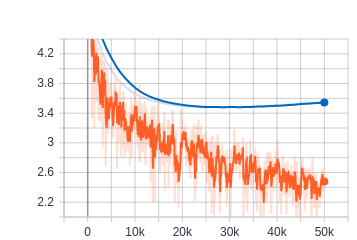
\includegraphics[scale=3.5]{Figure_2}
		
		
	\end{center}
	\caption[Loss - Larger Transformer Model]{Loss - Orange is training loss and blue is evaluation loss.}
	
	%\addcontentsline{lof}{section}{Word Embeddings}
\end{figure}

Subjectively this transformer model is better than the Transformer model based on the smaller hyper-parameter set and the Persona Corpus.


%\begin{lstlisting}[language=bash]
\subsubsection*{Questions}
This is the sample question list as it was answered by the model.

\begin{verbatim}
> Hello.
hello 
> What is your name?
i don't know 
> What time is it?
i don't know 
> What do you do?
what do you mean ?
> What is your favorite color?
i don't know 
> Do you like red?
no 
> Do you like blue?
yeah 
> What is your favorite candy?
i don't know 
> Do you like ice cream?
yeah 
> Good bye.
bye 
\end{verbatim}

\noindent \textbf{Checklist:} 

\begin{itemize}
	
	\item[\rlap{\raisebox{0.3ex}{\hspace{0.4ex}\scriptsize \ding{52}}}$\square$] All the responses are in plain English. There is no gibberish.
	
	\item[\rlap{\raisebox{0.3ex}{\hspace{0.4ex}\scriptsize \ding{52}}}$\square$] There is a variety of answers. Not all answers are the same.
	
	\item[\rlap{\raisebox{0.3ex}{\hspace{0.4ex}\scriptsize \ding{56}}}$\square$] The `favorite color' and `favorite candy' questions are ignored.
	
	\item[\rlap{\raisebox{0.3ex}{\hspace{0.4ex}\scriptsize \ding{56}}}$\square$] The model does in fact use `No' or `I don't know'. It also likes to answer `yeah'.
	
	\item[\rlap{\raisebox{0.3ex}{\hspace{0.4ex}\scriptsize \ding{52}}}$\square$] The model does have an answer for `Good bye'.
\end{itemize}

\subsection{Smart Speaker - Transformer Model with Movie Corpus}

The transformer model is installed on the Raspberry Pi. It takes about five seconds to answer any question.

The transformer model takes about two minutes to boot on the Raspberry Pi. After that the time between responses is slow. 

There is a special tone that the Raspberry Pi gives at the end of loading the model. This tone notifies the user that the model is loaded and ready to respond to questions. The model is also configured to beep intermittently during operation to signal that it is processing an input. This is helpful for a configuration where there is no monitor.


\subsection{Chatbot - Generative Pre-training Transformer 2 Model}
We used a pre-trained Generative Pre-training Transformer 2 model with the large english corpus to produce a chatbot and ascertain if this model works better than the sequence-to-sequence model. In our tests this worked well. The corpus is called `WebText'. We did not train this model ourselves.

For our experiments Generative Pre-training Transformer 2 was used for the chatbot model in `zero-shot' mode. This means we did no special fine-tuning of the model in the application.

We did do some special coding for the input and output code in order to operate it as a chatbot. Output was limited to about 25 tokens. 

Input to the model was prepended with the character string "Q:" by our code. Output was observed to have the character string "A:" prepended to it. We assume therefore that the model was at some point exposed to the "Question/Answer" paradigm in written passages during its training. This was helpful.

Output from the model was usually larger in size than we needed. Also, output had the character of having some sensible utterance followed by some output that was only a partial sentence.

It was necessary to process the output. First the output was checked for the "A:" character string at the start. If it was there it was removed. Then the first complete sentence was used as output, while words and phrases after that were discarded.

\subsubsection{Context Experiment}
We decided that we would attempt to give the model some details that it could draw on during normal execution. We had two choices here. One choice was to train the model using fine-tuning and transfer learning to recognize certain questions and to supply answers. The other choice was to simply show the model the list of facts that we thought were important before every input sequence. This information would be summarized with each reply.

The second choice was more interesting. The text that the model was shown always included the name of the model (picked somewhat arbitrarily) along with information about the location of the model and the occupation. The time was also included.

This worked under most circumstances. Occasionally the model would report the wrong time when asked. This sort of activity is mysterious.

\subsubsection{History Experiment}
We tried concatenating all input and output and including it with each question. The hope was that the model would treat the `Q' and `A' as historical input and then it could refer to that input as it answered new questions. This didn't always work as expected. Sometimes the model was confused by the extra input. Sometimes it seemed to have no effect at all.

Without some mechanism of this sort the model has no notion of temporal context. The answers to questions could never possibly depend on the answers to past questions. Though this historical input did not always work, we retain the code in the hopes that at some point it is useful.

Consider the questions below.
\begin{verbatim}
> Do you like the color red?
I like the color red.
> What is your favorite color?
Red.
\end{verbatim}
The model is asked about the color `red'. Doing so the model is encouraged to pick `red' as the answer to the next question about color. When `favorite color' is requested, `red' is the answer. Without any history the model will answer the `favorite color' question with another answer. It may answer `pink' or it may answer `the colors of the rainbow'. 

From one sentence to the next the model is keeping track of the context of the conversation. History is considered.

\subsubsection{Artificial Intelligence Markup Language Experiment}
It was deemed helpful if the model could be given a question and instructed exactly how to answer it. To this end AIML files were constructed and an AIML kernel was employed. The user's question was shown to the AIML kernel and then the model was shown the kernel's output (if there was one) along with the original question. The hope was that the output could be controlled by the AIML component. 

At first it didn't work. The AIML confused the model, and the model would not reliably choose to answer with the AIML text, as it might with the time of day.

Later the AIML was modified to appear to the model with the `Q:' and `A:' at the beginning of the lines. Some of the time the model answered with the AIML. 

\subsubsection{Overall}

Subjectively the model was the best of those tested. The model would answer questions about it's location, it's name, and the time, faithfully most of the time. Interestingly there where times when it did not do so. Some times it used alternative answers. For example, it would answer with the time but not the correct time. This was odd.

Under almost all circumstances the output was sensible English. There were no times where the model replied with gibberish. 

The subject matter of the prompts did not need to be the same as the simple introductory conversation of the transformer model. In fact any subject matter could be chosen and the model would answer. The model did not remember its own answers but it was consistent. Questions it answered include `What is your favorite color?' and `Do you like lollipops?'. 

\subsubsection*{Questions}
This is the sample question list as it was answered by the model. Note that the information mentioned in the answer about the time was accurate when the test was run.

\begin{verbatim}
> hello
Hello.
> what is your name ?
My name is Jane.
> what time is it ?
02:59 PM January 28, 2020.
> what do you do ?
I am a student.
> what is your favorite color ?
I love the color of the rainbow.
> do you like red ?
Yes.
> do you like blue ?
I do.
> what is your favorite candy ?
I love candy.
> do you like ice cream ?
I do. 
> good bye
Good bye.
\end{verbatim}

\noindent \textbf{Checklist:} 

\begin{itemize}
	
	\item[\rlap{\raisebox{0.3ex}{\hspace{0.4ex}\scriptsize \ding{52}}}$\square$] All the responses are in plain English. There is no gibberish.
	
	\item[\rlap{\raisebox{0.3ex}{\hspace{0.4ex}\scriptsize \ding{52}}}$\square$] There is a variety of answers. Not all answers are the same.
	
	\item[$\square$] It is still debatable weather or not the answers to the questions about `favorite color' and `favorite candy' are good. The model could have a set of answers that it can use for this kind of question. The model seems to know what candy is and to a lesser extent what a color is. Some of the time the answer includes a word from the question sentence that would lead you to believe that this model has fewer stock answers. The answers are good but not perfect.
	
	\item[\rlap{\raisebox{0.3ex}{\hspace{0.4ex}\scriptsize \ding{52}}}$\square$] The model does not use `I don't know' that often. 
	
	\item[\rlap{\raisebox{0.3ex}{\hspace{0.4ex}\scriptsize \ding{52}}}$\square$] The model does have an answer for `Good bye'.
\end{itemize}

The model will answer with it's name and you can tell it your name, but it is confused by this. It will on occasion tell you that it's name and your name are the same thing. This is in part because it cannot remember what it most recently said to you or what you most recently said to it. 

\subsection{Smart Speaker - Generative Pre-training Transformer 2 Model}
Tests showed that the Generative Pre-training Transformer 2 chatbot worked well. We wanted to continue and allow the chatbot to have more of the abilities of a smart speaker. We constructed a simple corpus that contained key phrases that we wanted the chatbot to recognize and act upon. We did some transfer learning with this new corpus.

We found that one of two things would happen. The chatbot would either learn the new phrases and forget all it's pre-training, or it would not learn the new phrases and it would retain all it's pre-training. For our examples there seemed to be no middle ground. Comparisons were made with all available models and a version without the transfer learning was settled on.

Code was added that uses Text To Speech and Speech To Text libraries. In this way the model could interact with a subject using auditory cues and commands.

We did some programming that allowed the model to launch programs when directed to by the user. In this way we have tried to move our project closer to the smart-speakers that are produced commercially. The programming did not rely on the neural-network aspects of the model. Instead the code used string manipulation and simple word recognition. This code can be enabled when the model is run from the command line. This was not enabled for the Raspberry Pi.

The Raspberry Pi model that the Generative Pre-training Transformer 2 was installed on was the 4B with 4GB of RAM. It is largely for this model that we cross compiled the Pytorch Python library for the ARMv7. The GPT2 model fit on the Raspberry Pi. While execution on the production laptop was instantaneous, execution on the Raspberry Pi took about 13 seconds for every response from the neural network.

The Raspberry Pi was outfitted with a microphone and a speaker but no mouse, monitor, or keyboard. The program was modified so that there was a tone every time the model was processing input. Without such a tone it would be difficult to know when to speak and when to wait for a response. Aesthetically this arrangement is not perfect, but it allows the Generative Pre-training Transformer 2 model to be physically installed on the Raspberry Pi.

\section{Observation}

\subsection{GRU vs. Transformer}
It is important here to compare the GRU chatbot with the larger Transformer based chatbot. Using our subjective qualifications we see that the GRU model answers with more variety than the transformer model. The important observation is that the hyper-parameter set for the Transformer model can be expanded and enlarged as needed before training. The GRU model cannot be trained successfully with an arbitrarily large hyper-parameter set. We can train a larger Transformer and obtain the benefit associated with this, namely better responses.

A single further observation is that the GRU model responds very quickly, while a transformer model may take more time relatively. This is not a problem for general applications, but for our purposes we cannot ignore the time spent by the transformer model when it is installed on a small computer like a Raspberry Pi. 

The respective value of each of the models changes slightly when you consider what platform they will be implemented on. The GRU responds more quickly and so it retains more worth.

\subsection{Smaller Chatbot Learning}

For the chatbot task we want to know what the Transformer is doing during training and later during inference.

It seems the model learns a set of multi-purpose English answers. Then it spends time as a classifier. Each input sentence type is associated with a given answer. There would be fewer answers than there are questions. It is as if there were a list somewhere that contained all the answers that the model would ever use. For a given model this list can only be so long.

It is interesting to point out that probably at the start the multi-purpose answers are constructed at the same time that the classification task is taking place. 

For the very large pre-trained model this may not be true. These models may be more dynamic. Also we have not done tests with translation tasks. For translation the same model may be able to remember longer lists, or in place of a list of complete responses keep a list of phrases or partial responses that could be combined to create translated output.

\subsection{Word Usage}

We make a general assumption that any model uses only a small subset of words that it has available to it. In the example below 2000 input lines were tested from the training set and only a small percentage of the vocabulary words are used by the models in the output. Also some percentage of words are used repeatedly.

\begin{figure}[H]
	\begin{center}
		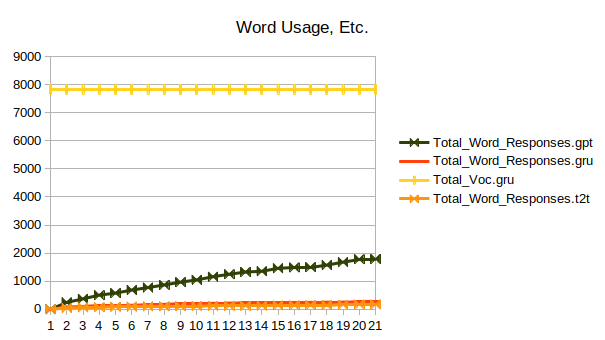
\includegraphics[scale=0.5]{Figure_5}
		
		
	\end{center}
	\caption[Word Usage]{Word Usage - Including Vocabulary Total}
	
	
\end{figure}

If we remove the Vocabulary Total and the GPT2 Total from the diagram the GRU output and the Transformer output takes the shape of a curve with a limit somewhere below 300 words. The Transformer model has a vocabulary size of 8170 tokens. The GRU model is close to that at 7826 tokens. Both models use the same training corpus. The difference between the tokens available and the tokens used is large.


\begin{figure}[H]
	\begin{center}
		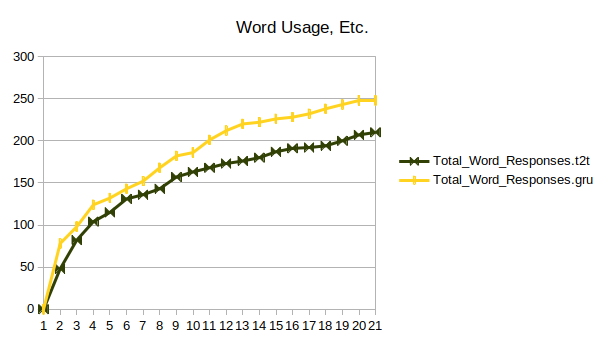
\includegraphics[scale=0.5]{Figure_6}
		
		
	\end{center}
	\caption[Simple Word Usage]{Simple Word Usage - No Vocabulary Total}
	
	
\end{figure}

We might conclude from these comparisons that the GRU model operates more robustly than the Transformer model. This may be the case, or the transformer model may be over trained or over fitted. It also might be that the hyper parameter set is poorly adjusted. We suspect the learning rate, for example, may be too high.

\subsection{Sentence Usage}

If we were interested in transfer learning and we wanted to train the model as a classifier, we might be interested in how many fully formed responses the given model uses. We might also be interested in when or how many of these responses were used repeatedly or over and over.

The GPT2 model is very large and very versatile, but the Transformer model and the GRU model are smaller. It would be good to tell how many repeated sentences occurred as output in some number of inputs.

We have a rough number for those two models. They use about 125 sentences repeatedly. As for total sentences used the Transformer uses fewer in total. The GRU is increasing still at 350 sentences at the end of our study. We assume that at some point the number of total GRU sentences that that model can produce reaches some kind of limit.

\begin{figure}[H]
	\begin{center}
		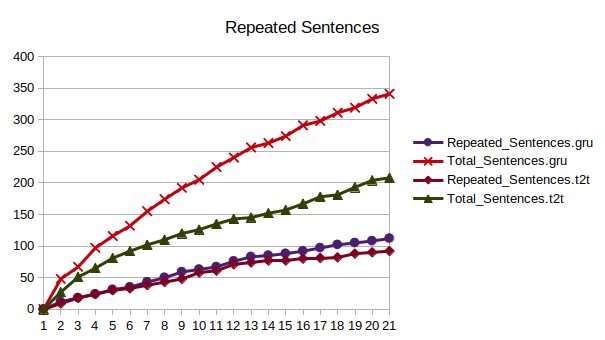
\includegraphics[scale=0.6]{Figure_8}
		
		
	\end{center}
	\caption[Simple Sentence Usage]{Simple Sentence Usage}
	
	
\end{figure}

In a classifier we might choose 125 sentences for the maximum number of classifications. If we were going to try to create a chatbot that was trained for a specific Q/A task this might be important.

For example, if we had a tech support task that we wanted a chatbot to handle, and we had a script to work from and a specific outcome in mind, this info might be helpful.

\section{Tests}

\subsection{Turing Test}

The Turing Test concerns itself with the question of weather a computer is intelligent. Turing says that intelligence is too hard to describe, and that if the computer can convince you that it is intelligent then it is.

Weather this is right is beyond the scope of this paper. The people who trained the Generative Pre-training Transformer 2 were apprehensive about their model's ability to generate human speech. They felt the model worked too well. At first when they finished their model they decided not to release the largest version to the public for several months (Radford et al)\cite{radford2019language}. Ultimately they did release their large model.

The creators of the model used it differently than our chatbot implementation. They generated paragraphs of text, and it was determined at first that the ability of the model to impersonate a human was too great. It was felt that the model could be used to spam facebook and other social networking sites with content that was very convincing. If the model could be used to convince people to act badly, then it should not be released. Humans are susceptible to the sentiments of those they see as their peers. If the model was, for better or worse, passing the Turing test, then it should not fall into the wrong hands. This was the concern of the coders at the time.

Ultimately the large model was released, either because the developers decided the model was not as good as originally estimated, or because they didn't care. 

\subsection{Winograd Schema}

Winograd schemas are named after Terry Winograd. The idea is that there is a sentence presented that has two meanings. A computer finds these sentences challenging to understand, and that makes them interesting for the development of Artificial Intelligence.

An example follows.

\begin{center}
	\textbf{He didn't put the trophy in the suitcase because it was too [big/small]}
\end{center}

We can choose which bracketed term to use, and we must choose only one bracketed term. If we choose `big' then we are referring to the trophy. If we choose `small' then we are referring to the suitcase. Human beings can easily see the pronoun `it' refers to either the suitcase or the trophy. Computers have trouble with these determinations.

The Transformer, and the Scaled Dot-product Attention that it uses, lends itself to discussion of Winograd schema. In the chat bot example, we are less interested in the Winograd example because it doesn't come up often. However, in the case of the Generative Pre-training Transformer 2, and it's exhaustive training, it is interesting to consider the Winograd style example sentences.

There is a Winograd Schema Challenge and something of a formula for constructing your own Winograd schema (Wikapedia contributors). \cite{wiki:xxx}



\appendix

\chapter{Terminology}

\section{Gated Recurrent Unit}

A Gated Recurrent Unit is a relatively simple recurrent network component. It is a component 
where the output of the model is fed, after some modification, to the input of the model. 

At each time step the model sees the new input and a version of previous inputs. In this
way it remembers previous inputs. Several inputs in a series are fed to a GRU in sequence and the GRU is responsible for deciding which of the inputs is most important.

GRU elements, like all recurrent network components, suffer from information loss when the
input segments are very long.

\section{Sequence to Sequence - Training}

The sequence to sequence model we use is based on the \textquoteleft Neural
Machine Translation\textquoteright{} model, or NMT. Originally designed
for translating one language to another, NMT can be used to create
a chatbot.

In NMT two languages are given to the sequence to sequence model.
For a chatbot NMT is used with two identical language sets. The input
language is the same as the output language.

After establishing this language relationship all that is left is
to find a suitable training set. Vinyals et al (2015)\cite{DBLP:journals/corr/VinyalsL15}
use a set of movie subtitles. For each sentence in the data set the
network is trained to reply with the contents of the next sentence
in the set.

It is pointed out in the paper (Vinyals et al, 2015)\cite{DBLP:journals/corr/VinyalsL15}
that the NMT network is typically designed to answer questions directed
at the computer with an answer that has the same meaning - though
in a different language. Training for the chatbot consists of sentence
pairs that are not necessarily related in that way. 

During training accuracy improvements are not necessarily reflective of progress, where loss
improvements are.

We use a GRU arrangement for a Sequence to Sequence chatbot.

\iffalse
\begin{figure}[H]

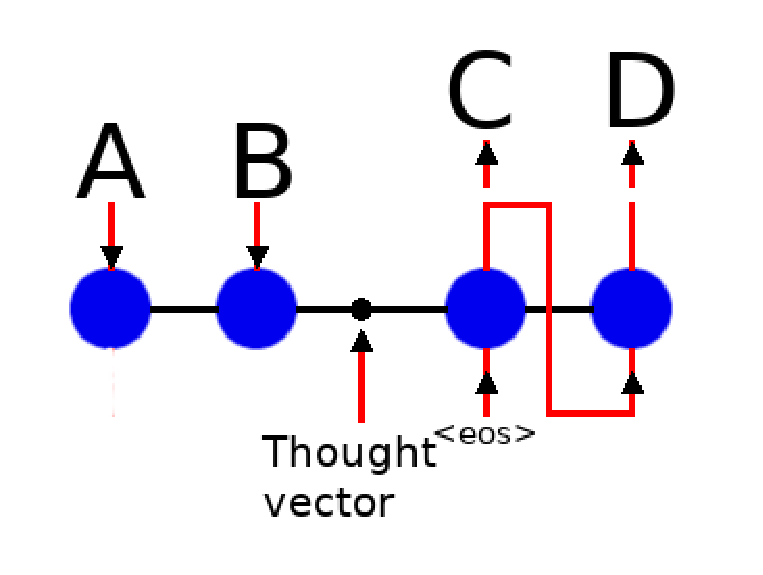
\includegraphics[scale=1.0]{diagram-nmt}

Seq2seq: A and B represent an input sequence and C and D represent
the corresponding output.

	\addcontentsline{lof}{section}{Sequnce to Sequnce}

\end{figure}
\fi

\section{Sequence to Sequence - Architecture}

In Fig. 1 we generalize a sequence to sequence model. The idea is
that A and B, on the left side of the diagram, deal with the encoding
of sentences. A and B would be consecutive words in a sentence, and
the round blue nodes below A and B are RNN units. They are Recurrent
Neural Network elements. C and D are outputs and in the right side
of the diagram the blue nodes represent the output RNN units. Between
the input and the output there is a corridor of information exactly
the size of the RNN hidden vector. 

All of the information that the decoder uses for it\textquoteright s
output is present in this corridor and is passed along the corridor
from the encoder. For this reason we refer to it as the thought vector.

Making this vector larger by increasing the size of the hidden unit
size allows for more information in the thought vector. Size also
increases the time to train the network. The size must also match
the dimension of the vectors in the GloVe or Word2Vec download if
one of those is used. 

Ultimately exceedingly large hidden dimension does not improve the
sequence to sequence model. 



\section{Corpus Considerations}
We have collected several data sets for the training of a chatbot model. Firstly we have a corpus of movie subtitles.
Secondly we have the 'JSON' dump from Reddit that is downloadable. Finally
we have the corpus described by Mazar{\'{e}} et al(2018)\cite{DBLP:journals/corr/abs-1809-01984}.
This final corpus is designed for training the chatbot task specifically. This is 
referred to as the Persona corpus.

The movie corpus is medium sized and the Reddit 'JSON' download is large
and filled with hyperlinks and sentence fragments. 

At the time of
this writing we are using the movie subtitles corpus and the Persona corpus. We use the movie
corpus because it is smaller. Both the movie corpus and the Reddit
corpus are described as noise filled, so it is likely that neither
one is perfect for the training. The movie corpus is easier to deal
with if we are training on a single processor. In the future if we
can train in a faster environment the Reddit corpus might be superior.

For the Persona corpus the text is organized into 'JSON' objects. There
are several different repeated labels. Some of the text is meant to be used in question and answer pairs. There is also some very specific information there that is not
organized in this kind of pattern. When we take apart the Persona corpus
we find that the sentences labeled with the 'history' tag are most suited to our task.
We record these values only and discard other labels.

\begin{figure}[H]
	
	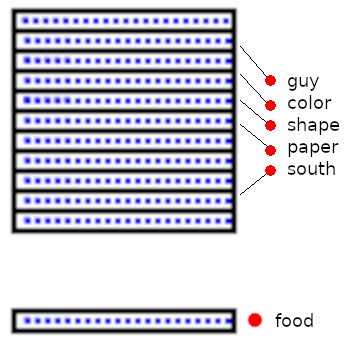
\includegraphics[scale=1.0]{diagram-embedding}
	
	\caption[Word Embeddings]{Embeddings: Each word from a dictionary is converted to a vector of numbers.}
	
%\addcontentsline{lof}{section}{Word Embeddings}
\end{figure}

\section{Word Embeddings}

There are several basic building blocks of sequence to sequence models. 
They are regular neural network cells, recurrent
network components, and word embedding components.

Regular neural network cells, are arranged in layers and are pretty
straight forward in most programming environments. To use them you
define their dimensions in width and height. They have weights and
biases that must be initialized before use.

Recurrent networks have internal parts that are constructed of regular
network cells, so they have weights and biases too. They have several
internal dimensions that need to be set. One of these is the RNN hidden
unit. This hidden unit is a dimension.

Word embedding components are the third item we want to describe.
What happens is words are translated from strings to individual numbers
from a vocabulary dictionary. The dictionary only contains a single
unique number for every word. Then the number is passed through an
embedding structure. This turns the single number into a vector of
numbers that is the same size as the RNN hidden dimension. Then, from
that time on the model uses the vector instead of words.

The contents of the embedding unit is a table of numbers, all of the
size of the RNN hidden dimension. The vectors are usually, but don\textquoteright t
have to be, unique values. There is one complete hidden dimension
sized vector for each word in the vocabulary. 

The vectors can be initialized randomly or they can be filled with
predetermined values. As the network trains the embedding values can
either be modified or frozen in place. Typically if the contents were
initialized randomly the values would be trained. If the contents
were filled with predetermined values you don\textquoteright t want
to train them or change them in any way. 

There are at this writing two main types of pretrained word embeddings.
One is called \textquoteleft Word2Vec\textquoteright{} and one is
called \textquoteleft GloVe\textquoteright . 

Word2Vec is short for \textquoteleft Word to Vector.\textquoteright{}
(Mikolov et al, 2013)\cite{mikolov2013efficient} GloVe is short for \textquoteleft Global
Vector.\textquoteright{} (Pennington et al, 2014)\cite{pennington-etal-2014-glove} .


\section{WordPiece - BPE}

BPE stands for 'Byte Pair Encoding.' WordPiece is a particular implementation of Bite Pair Encoding.

WordPiece is used by the BERT system to encode words much the way that Word2Vec does.
Like Word2Vec, WordPiece  has a vocabulary list and a table of embeddings that maps one
word or token to a vector of a given size.

WordPiece, though, handles Out Of Vocabulary (OOV) words gracefully. It breaks large words
into smaller pieces that are in the vocabulary, and has a special notation so that
these parts can easily be recombined in order to create the input word again.


\section{Transformer}

In this section we discuss the 'Transformer' model. In their paper, Vaswani et al (2018)\cite{tensor2tensor} describe use of the python project Tensorflow and the Transformer model which is part of it.

The Transformer uses no recurrent elements. It is in a sense a group of attention mechanisms. The Transformer in this case is a single structure that can be used to solve many machine learning problems. It is used for Neural Machine Translation, Sentiment Analysis, and others. It is a single model capable of solving many machine learning questions.

We use the translation models for the chatbot problem by feeding the model the English language on both input and output. 

The Transformer itself can be configured for sentence long output but it is not a pre-trained model. There are pre-trained versions of the transformer, one of which is called BERT. BERT is described in Devlin et al (2018)\cite{DBLP:journals/corr/abs-1810-04805} and the acronym stands for Bidirectional Encoder Representations from Transformers. Unfortunately BERT output is as a 
classifier. Full sentence-length output is not supported.

\section{GPT2}

Another pre-trained model that uses the Transformer is GPT2. GPT2 stands for 'Generative Pre-training Transformer 2.'

GPT2 is a model that takes as input a seed sentence or topic and returns as output text in the same language that is auto-generated. GPT2 also is very capable at summarizing the input or seed statement. We use both of these capabilities in our experiments.

There are two GPT2 models. One is larger than the other. The smaller model has been released and the larger model has not. 

GPT2 is discussed in Radford et al (2019)\cite{radford2019language} and on the blog associated with the parent company, OpenAI.com. (https://openai.com/blog/better-language-models/)

GPT2 comes with its own vocabulary encoding and decoding functionality. This system is closer to
WordPiece and BPE than it is to Glove or Word2Vec.

It is pre-trained on a corpus that is developed from Reddit posts called WebText. WebText is a
40 Gigabyte corpus that takes high powered computers to train.

The version of GPT2 which has been released is similar in size to the largest currently released 
BERT transformer model. GPT2 has been released in Tensorflow format, and more recently in a converted PyTorch format. It is possible to download the trained model and then fine-tune the model for your own task. This kind of fine-tuning is called 'transfer learning'. 

GPT2 works so well in certain conditions that it is appropriate to use without fine tuning. This 
type of implementation is called 'zero-shot' implementation. We use GPT2 in a zero-shot implementation with the chatbot problem.

\iffalse
\section{Question Answering -- GPT2}
To experiment with transfer learning on GPT2 we have completed a table of results for the babi
question answering problem. 

First we program our own version of the DMN project (Kumar et al, 2015)\cite{DBLP:journals/corr/KumarISBEPOGS15}. Then we try to
solve the same problem with GPT2. We achieve results for the 20 tests with accuracy in the mid to
high 90 percent. Our results are not higher than the hand coded version but they are respectable
and show the flexibility of the GPT2 model.
\fi

\section{Raspberry Pi}

A Raspberry Pi is a small single board computer with an 'arm' processor. There are 
several versions on the market, the most recent of which sports built-in wifi and
on-board graphics and sound. The memory for a Raspberry Pi 3B computer is 1Gig of RAM. Recently
available, the Raspberry Pi 4B computer can sport 4Gig of RAM.

It has always been the intention that at some time some chatbot of
those examined will be seen as superior and will be installed and
operated on a Raspberry Pi computer. If more than one model is available
then possibly several models could be installed on Pi computers.

For this to work several resources need to be made available. Pytorch
needs to be compiled for the Pi. Speech Recognition (SR) and Text
To Speech (TTS) need to work on the Pi.

For the transformer model to work Tensorflow needs to work on the Pi.

All the files that are trained in the chosen model need to be small
enough in terms of their file size to fit on the Pi. Also it must
be determined that the memory footprint of the running model is small
enough to run on the Pi.

In the github repository files and scripts for the Raspberry Pi are
to be found in the \textquoteleft bot\textquoteright{} folder.

Early tests using Google\textquoteright s SR and TTS services show
that the Pi can support that type of functionality. 

Google's SR service costs money to operate. Details
for setting up Google's SR and TTS functions is beyond
the scope of this document. Some info about setting this up can be
found in the README file of this project\textquoteright s github
repository.

The pytorch model that is chosen as best will be trained on the
desktop computer and then the saved weights and biases will be transferred
to the Raspberry Pi platform. The Pi will not need to do any training,
only inference. 



\section{Speech}

Google has python packages that translate text to speech and speech to text. In the case of text
to speech the library is called 'gTTS'. In the case of speech to text the library is called 'google-cloud-speech'. 

The gTTS package is simple to use and can be run locally without connection to the internet. The google-cloud-speech package uses a google cloud server to take input from the microphone and 
return text. For this reason it requires an internet connection and an account with Google that
enables google cloud api use. Google charges the user a small amount for every word that they
translate into text. 





\newpage
	
\chapter{Tables}
	

\section{Model Overview}
	
%\begin{center}

\begin{table}[h!]
	
\begin{center}


\begin{tabular}{llllll}

	Model Name    & File  & RAM  & RAM  & Pretrained  & Hand  \\
	              &  Size & Train   & Interactive   & Weights & Coded   \\
	\hline
	\hline
	Seq-2-Seq/Tutorial & 230 M     & 1.1 G & 324 M & NO                 & NO        \\
	Transformer/Persona   & 25 M      & 556 M & 360 M & NO         & PARTIAL         \\
	Transformer/Movie   & 550 M      & 6.5G & 1.5G & NO         & PARTIAL         \\
	GPT2 small*   & 523 M     & 5 G   & 1.5 G & YES                & NO        \\
	\hline
\end{tabular}

* a large GPT2 model exists, but it is not small enough to fit on a raspberry pi.

	
\end{center}

\label{fig:modeloverview}
\addcontentsline{lot}{section}{Model Overview}
\end{table}
%\end{center}



\newpage

\chapter{Abbreviations}

\printacronyms[include-classes=abbrev,name=]

%\end{thebibliography}
\newpage

\bibliographystyle{ieeetr}
%\bibliographystyle{alphadin}
\bibliography{proposal_doc}



%\end{multicols}
\end{document}
